%\documentclass[12pt,a4paper]{report}
%\usepackage[utf8]{vietnam}
%\usepackage{amsmath}
%\usepackage{amsfonts}
%\usepackage{amssymb}
%\usepackage{graphicx}
%\usepackage[left=2cm,right=2cm,top=2cm,bottom=2cm]{geometry}
%
%
%\usepackage{algorithm}
%\usepackage{algorithmic}
%\usepackage{mathtools}
%\setcounter{secnumdepth}{4} % multi-level
%\setcounter{tocdepth}{4}
%
%\usepackage{subfig}
%\usepackage{hyperref}
%
%\usepackage{tabularx}
%\begin{document}
\everymath{\displaystyle}  
\chapter{Cơ Sở Toán Học}
\label{chap:chap3}
\section{Ma trận}
\subsection{Định nghĩa}
 Một ma trận \textbf{A} loại (cấp) $m_x n$ trên trường $\mathbb{K}$ ($\mathbb{K}$ – là trường thực $\mathbb{R}$ hoặc phức $\mathbb{C}$) là một bảng chữ nhật gồm $m x n$ phần tử trong $\mathbb{K}$ được viết thành $m$ dòng và $n$ cột như sau:
\begin{align*}
	\begin{bmatrix}
		a_1{}_1 & a_1{}_2 & a_1{}_3  &\ldots& a_1{}_n \\
		a_2{}_1 & a_2{}_2 & a_2{}_3  & \ldots & a_2{}_n \\
		a_3{}_1 & a_3{}_2 & a_3{}_3  & \ldots & a_3{}_n \\
		\vdots & \vdots& \vdots  & \ddots& \vdots\\			
		a_m{}_1 & a_m{}_2 & a_m{}_3 &\ldots& a_m{}_n \\
	\end{bmatrix}	
\end{align*}
Trong đó: \\ 

	 $a_{ij}$ là phần tử của ma trận A nằm ở giao điểm của dòng i và cột j\\
	
	 m : số dòng của ma trận \textbf{A}\\
	
	 n: số cột của ma trận \textbf{A}\\
	
	 
$	\begin{bmatrix}
		a_{i1} & a_{i2}& a_{i3}&\ldots& a_{in}			
	\end{bmatrix}$ : 
	dòng thứ i của ma trận \textbf{A}\\
	
	
	$\begin{bmatrix}	
		 a_{j1} \\ a_{j2}\\ a_{j3} \\ \vdots \\ a_{jm}		\end{bmatrix}$ : 
	  cột thứ j của ma trận \textbf{A}\\

\subsection{Phép cộng ma trận}
 Cho hai ma trận \textbf{A}, \textbf{B} cùng cỡ  $ m_x n$, ta có tổng $\textbf{A} + \textbf{B}$ là ma trận có cùng kích thước ($m_x n$) với phần tử trong vị trí tương ứng bằng tổng của hai phần tử tương ứng của mỗi ma trận:
\begin{center}
$(\textbf{A}+\textbf{B}) = a_{ij}+b_{ij}$ với $ 1 \leq i \leq m$ và $1 \leq j \leq n$

\end{center}

Ví dụ:

$\begin{bmatrix}
   1 & 2 \\6 & 3
\end{bmatrix}$
+ 
$\begin{bmatrix}
3 & -2 \\
-4 & 1
\end{bmatrix}$
=
$\begin{bmatrix}
1+3 & 2 + -2 \\
6+-4 & 3+1
\end{bmatrix}$
=
$\begin{bmatrix}
4& 0\\
2 & 4
\end{bmatrix}$


\subsection{Phép nhân ma trận với ma trận}
Xét ma trận $\textbf{A}_m{}_x{}_p$ và ma trận \textbf{B}$_p{}_x{}_n$, trong đó số cột của ma trận \textbf{A} bằng số hàng của ma trận \textbf{B}.
 Tích \textbf{A}\textbf{B} là ma trận \textbf{C} có m hàng và n cột, phần tử $c_i{}_j$ được xác định theo tích vô hướng của hàng tương ứng trong \textbf{A} với cột tương ứng trong \textbf{B}: 
\begin{align*}
c_i{}_j = a_i{}_1b_j{}_1 + a_i{}_2b_j{}_2 + \ldots + a_i{}_pb_j{}_p=
\sum_{k=1}^p(a_{ik}b_{jk})
\end{align*}


Ngoài ra có một phép nhân khác được gọi là \textit{element-wise} (hay \textit{hadamard}) được sử dụng khá nhiều trong học máy. Tích element-wise của hai ma trận cùng kích thước A, B được kí hiệu là $\textbf{C}=\textbf{A} \odot \textbf{B}$, trong đó:
\begin{equation*}
c_{ij}=a_{ij}b_{ij}
\end{equation*}
\subsection{Ma trận chuyển vị}
 Ma trận chuyển vị là một ma trận ở đó các hàng được thay thế bằng các cột, và ngược lại hay nói cách khác nếu ma trận \textbf{B} là ma trận chuyển vị của ma trận \textbf{A} thì: $b_{ij} = a_{ji}$ \par
Ma trận chuyển vị của ma trận $\textbf{A}$ được ký hiệu là $\textbf{A}^T$.\\ \par

$\begin{bmatrix}
a & b\\ c&d
\end{bmatrix}^T$
=
$\begin{bmatrix}
a&c\\b&d
\end{bmatrix}$
\section{Đạo hàm}
\subsection{Định nghĩa}
 Cho hàm số ${ y=f(x)}$ xác định trên khoảng ${ (a;b)}$ (khoảng ${  (a;b)=\{x\in \mathbb {R} |a<x<b\}}$. Xét giá trị ${  x_{0}}$ và giá trị ${  x\in (a;b),x\neq x_{0}}$. \par 

Đặt $   \Delta x=x-x_0$ thì $  x = x_0+\Delta x$ và $\Delta x$ được gọi là số gia đối số. \par

Đặt $  \Delta y = f(x)-f(x_0)$ và $\Delta y$ được gọi là số gia hàm số. \par

Xét tỷ số ${  {\frac {\Delta y}{\Delta x}}}$. Nếu khi $  \Delta x\rightarrow0$, tỷ số đó dần tới một giới hạn thì giới hạn đó được gọi là đạo hàm của hàm số $  y=f(x)$ tại điểm $  x_0$ ký hiệu là ${  f'(x)}$\\

${  f'(x)=\lim _{\Delta x\rightarrow 0}{\frac {f(x_{0}+\Delta x)-f(x_{0})}{\Delta x}}}  $
\subsection{Đạo hàm riêng}
Đạo hàm riêng của một hàm số đa biến là đạo hàm theo một biến, các biến khác được xem như là hằng số. \par
Đạo hàm riêng của f đối với biến x được ký hiệu khác nhau bởi : ${  f'_x }$,  ${  \frac{\partial f}{\partial x} }.$\par
Ví dụ: Hàm số $f(x,y) = ax^2 + bxy + cy^5$ thì ta có:
\begin{itemize}
\setlength{\itemindent}{10mm}
	\item Đạo hàm theo x: ${  f'_x = 2ax +by}$
	\item Đạo hàm theo y: ${  f'_y = bx +5cy^4}$	
\end{itemize}

\textbf{Vector gradient}:
Cho một hàm số $f(\textbf{x})$ : $\mathbb{R}^n \rightarrow \mathbb{R}$. Trong trường hợp này f có các đạo hàm riêng $   \frac{\partial f}{\partial x_j}$ đối với mỗi biến $ x_j$ ($1\leq j \leq n$) thì vector chứa các đạo hàm riêng này là vector gradient.\par
\begin{center}

$ \nabla_\textbf{x}f(\textbf{x}) =
\renewcommand{\arraystretch}{2.5} 
\begin{bmatrix}

\frac{\partial f(\textbf{x})}{\partial x_1}\\ \frac{\partial f(\textbf{x})}{\partial x_2} \\ \vdots \\ \frac{\partial f(\textbf{x})}{\partial x_n}
\end{bmatrix}  $
\end{center}

\subsection{Đạo hàm hàm hợp (Chain rule)}

 Đạo hàm hàm hợp là công thức để tính đạo hàm của hàm số gồm nhiều hàm số kết hợp với nhau. Đó là, nếu $f, g$ là hai hàm số và hàm $h(x) = f(g(x))$ thì ta có 
\begin{center}
$h'(x) = f(g(x))' = f'(g(x)).g'(x) $

\end{center}
hay chúng ta có công thức quen thuộc hơn với cách đặt $z=f(y), y=g(x)$:
\begin{center}
$\frac{dz}{dx} = \frac{dz}{dy} \frac{dy}{dz}$ = $f'(y)g'(x)$ = $f'(g(x)).g'(x)$
\end{center}

%Ví dụ: Tính đạo hàm của hàm số $h=(x^2+5)^2$\par
% Đặt $g(x) = x^2 +5$ thì ta có $f(g) = g^2$, do đó $h'(x) = f'(g(x)).g'(x) = 2g2x= 4(x^2 +5)x$\par
%\textbf{Đạo hàm riêng của hàm hợp}: Giả sử ta có hàm số $f(u,v)$ trong đó $u(x,y)$ , $v(x,y)$ là các hàm số  theo biến $x,y$ và $f$ có đạo hàm riêng theo $u,v$ và $u,v$ có đạo hàm riêng theo $x,y$ thì ta có đạo hàm riêng của $f$ theo $x,y$ như sau:
%\begin{align*}
%	\begin{cases}
%        f'_{x} = f'_{u}u'_{x} +f'_{v}v'_{x}\\
%       f'_{y} = f'_{u}u'_{y} +f'_{v}v'_{y}
%    \end{cases}
%\end{align*}
%một cách biểu diễn khác
%\begin{align}
%	\begin{cases}
%		\frac{\partial f}{\partial x} = 
%		\frac{\partial f}{\partial u}\frac{\partial u}{\partial x} + 
%		\frac{\partial f}{\partial v}\frac{\partial v}{\partial x}\\[5mm]
%		\frac{\partial f}{\partial y} = \frac{\partial f}{\partial u}\frac{\partial u}{\partial y} +
%		 \frac{\partial f}{\partial v}\frac{\partial v}{\partial y}
%	\end{cases}
%\end{align}
\section{Ước lượng tham số bằng cực đại khả dĩ}
 Ước lượng hợp lý cực đại (có người gọi là khả năng cực đại, tiếng Anh thường được viết là MLE, gọi tắt từ Maximum-Likelihood Estimation) là một kỹ thuật trong thống kê dùng để ước lượng giá trị tham số của một mô hình xác suất dựa trên những dữ liệu có được. Phương pháp này được đĩnh nghĩa như sau:\par
Giả sử $X=x_1,x_2,....,x_n$ là tập $n$ quan sát và $Y=y_1,y_2,...,y_n$ là số nhãn của quan sát; $x,y$ là hai biến độc lập ngẫu nhiên. Ta cần phải tìm tham số $\theta$ để biểu thức sau đây đạt được giá trị lớn nhất
\begin{equation}
\label{eq:ults}
h_{\theta} = P(Y|X;\theta)
\end{equation} 
hay biểu thức \ref{eq:ults} được viết lại như sau:
\begin{equation}
\widehat{\theta} = \arg\max_{\theta}P(Y|X;\theta)
\end{equation}
Do các quan sát là biến độc lập ngẫu nhiên nên ta có thể viết lại thành:
\begin{equation}
P(Y|X;\theta) = \prod^N_{i=1}P(y_i|x_i,\;\theta)
\end{equation}
Nhưng trực tiếp hàm số trên không hề đơn giản, hơn nữa khi N lớn thì tích của N số nhỏ hơn một có thể dẫn đến sai số trong tính toán. Một phương pháp thường được sử dụng đó là lấy logarit	tự nhiên (cơ số e) của hàm khả dĩ ta được:
\begin{equation}
l(P(Y|X;\theta)) = log\prod_{i=1}^N P(y_i|x_i;\theta)=\sum_{i=1}^NlogP(y_i|x_i;\theta)
\end{equation}
\section{Một vài phương pháp tối ưu}
\label{sec:toiuu}
 Mục tiêu của bài toán tối ưu là tìm ra nghiệm \textit{global minimum}(điểm mà tại đó hàm số đạt giá trị nhỏ nhất) của hàm số.  Tuy nhiên, việc tìm global minimum của các hàm số là rất phức tạp, thậm chí là bất khả thi. Thay vào đó, người ta thường cố gắng tìm các điểm \textit{local minimum} (điểm cực tiểu), và ở một mức độ nào đó, coi đó là nghiệm cần tìm của bài toán.\par
Giả sử ta có $N$ quan sát $(\textbf{X},\textbf{y})$ có ánh xạ $\textbf{X} \to \textbf{Y}$ với $f(\mathbf{\theta},\textbf{X})=\textbf{y}$. Ta cần tìm global minimum cho hàm $f(\theta;\textbf{X},\textbf{y})$ trong đó $\mathbf{\theta}$ là một vector, $\theta=[\theta_1,\theta_2,...,\theta_m]$. Đạo hàm của hàm số đó tại một điểm   $\mathbf{\theta}$ bất kỳ được ký hiệu là $\nabla_\mathbf{\theta} f(\mathbf{\theta};\textbf{x},y)$
\subsection{Gradient descent}
 Thuật toán gradient descent giúp ta tìm $\theta$ sao cho $f(\mathbf{\theta},\textbf{X})~\text{gần}~\textbf{y}$ nhất.
\begin{algorithm}[H]
\label{alg:grad}
\caption{Gradient desent}
\begin{algorithmic}[1]
\REQUIRE Tập $N$ quan sát (\textbf{X},\textbf{y})
\REQUIRE $\theta=[\theta_1,\theta_2,...,\theta_m]$
\REPEAT 
\FORALL {$i=1;i \leq N;i++$}
\STATE $\nabla \theta_i := - \nabla_{\theta}f(\theta;\textbf{x}_i,y_i)$
\ENDFOR
\STATE $\nabla \theta  =\frac{1}{N} \sum^{N}_{i=1}\nabla\theta_i$
\STATE Chọn bước nhảy $\eta$
\STATE Cập nhật $\theta := \theta - \eta\nabla\theta$

\UNTIL	thuật toán hội tụ
\end{algorithmic}
\end{algorithm}
Trong đó $\eta$ (đọc là eta) là một số dương được gọi là learning rate (tốc độ học) và giá trị của learning rate thường là 0.001. Việc lựa chọn learning rate rất quan trọng trong các bài toán thực tế. Việc lựa chọn giá trị này phụ thuộc nhiều vào từng bài toán và phải làm một vài thí nghiệm để chọn ra giá trị tốt nhất. Và dấu trừ tại $\nabla \theta := - \nabla_{\theta}f(\theta)$ thể hiện việc chúng ta phải đi\textit{ ngược với đạo hàm} (Đây cũng chính là lý do phương pháp này được gọi là Gradient Descent - descent nghĩa là đi ngược).\par
Nếu dữ liệu có kích thước $N$ lớn thì mỗi lần cập nhật $\theta$ đòi hỏi chúng ta sử dụng tất cả các quan sát $\textbf{x}_i$ do đó khối lượng tính toán lớn do phải tính đạo hàm trên toàn bộ dữ liệu, thuật toán chạy chậm. Do vậy để tiết kiệm khối lượng tính toán, chúng ta sẽ cập nhật tính toán sau mỗi dữ liệu quan sát, phương pháp này gọi là \textit{sochastic gradient descent (SGD)}

\begin{algorithm}[H]
\label{alg:sgd}
\caption{Stochastic Gradient descent}
\begin{algorithmic}[1]
\REQUIRE Tập $N$ quan sát (\textbf{X},\textbf{y})
\REQUIRE  $\theta=[\theta_1,\theta_2,...,\theta_m]$
\REPEAT 
\STATE Xáo trộn dữ liệu
\FORALL {$i=1;i \leq N;i++$}
\STATE $\nabla \theta_i := - \nabla_{\theta}f(\theta;\textbf{x}_i,y_i)$

\STATE Chọn bước nhảy $\eta$
\STATE Cập nhật $\theta := \theta + \eta\nabla\theta$
\IF {hội tụ}
	\STATE \text{break}
\ENDIF
\ENDFOR

\UNTIL	thuật toán hội tụ
\end{algorithmic}
\end{algorithm}
Khác với SGD, thay vì mỗi \textit{iteration} ta tính toán trên một quan sát thì ta sẽ tính toán với $k$ quan sát ($1<k\ll N$). Phương pháp này được gọi là \textit{mini-batch gradient descent.}

\begin{algorithm}[H]
\label{alg:minibatch}
\caption{Mini-batch Gradient descent}
\begin{algorithmic}[1]
\REQUIRE Tập n quan sát (\textbf{X},\textbf{y})
\REQUIRE $\theta=[\theta_1,\theta_2,...,\theta_m]$
\REPEAT 
\STATE Xáo trộn dữ liệu
\FORALL {$i=1;i \leq N;i=i+k$}
\STATE $\nabla \theta_i := -\sum^{i+k}_{j=i} \nabla_{\theta}f(\theta;\textbf{x}_j,y_j)$
\STATE Chọn bước nhảy $\eta$
\STATE Cập nhật $\theta := \theta - \eta\nabla\theta_i$
\IF {hội tụ}
	\STATE \text{break}
\ENDIF

\ENDFOR

\UNTIL	thuật toán hội tụ
\end{algorithmic} 

\end{algorithm}

\subsection{Gradient descents với Momentum}
  Giả sử ta vẽ được một thung lũng như Hình \ref{fig:dothi}, ta thả một viên bi vào trong đó và mong muốn nó lăn đến điểm B, điểm sâu nhất của thung lũng. Nếu ta may mắn thả viên bi ở điểm A hoặc điểm G thì viên bi dễ dàng đến tiến điểm B. Nhưng nếu ta thả viên vi tại điểm D thì viên bi có thể sẽ giao động xung quanh điểm E và dừng tại đó do chưa đủ lực để đẩy viên bi qua điểm F rồi đến điểm G. Khi đó E chính là một điểm local minimum mà chúng ta không muốn. Do đó nếu ta tác động thêm một lực vào viên bi giúp nó có thể từ điểm E vượt qua F và tiến đến G. 
\begin{figure}[H]
\begin{center}
\label{fig:dothi}
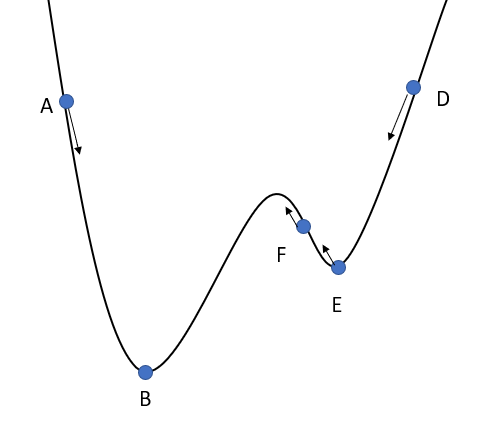
\includegraphics[scale=1]{chap3/image/momentum.png}
\caption{Đồ thị }
\end{center}
\end{figure}
Thuật toán gradient descent được ví như trọng lực tác dụng vào viên bi giúp nó di chuyển, B được coi điểm global minimum và E là một điểm local minimun. Để tránh hiện tượng nghiệm của gradient descent rơi vào một điểm local minimum không mong muốn thì ta tác động thêm một lực giúp gradient descent có thể bật ra khỏi vị trí của local minimum, lực này gọi là đà (\textit{momentum}). Vì thế cách cập nhật $\theta$ sẽ thay được thay đổi một chút như sau:
\begin{itemize}
\item[] $v_t:= \beta v_{t-1} +\eta \nabla\theta_{t}$
\item[]  $ \theta_t:= \theta_{t-1} - v_t$
\end{itemize}
Với $t$ là bước lặp thứ \textit{t}, biến $v$ được khởi tạo bằng 0 và trong tối ưu $\beta$ được gọi là đà (\textit{momentum}) với giá trị thường là $0.9$.
%\begin{algorithm}[H]
%\label{alg:momentum}
%\caption{Momentum kết hợp mini-batch}
%\begin{algorithmic}[1]
%\REQUIRE Tập n quan sát (\textbf{X},\textbf{y})
%\REQUIRE $\theta=[\theta_1,\theta_2,...,\theta_m]$
%\REPEAT 
%\STATE Xáo trộn dữ liệu
%\STATE v:=0
%\FORALL {$i=1;i \leq N;i=i+k$}
%\STATE $\nabla \theta_i := -\sum^{i+k}_{j=i} \nabla_{\theta}f(\theta;\textbf{x}_j,y_j)$
%\STATE $\mathit{v := mu*v+ \eta \nabla\theta_i}$
%\STATE Chọn bước nhảy $\eta$
%\STATE Cập nhật $\theta := \theta - v$
%\STATE if(hội tụ)
%\STATE break
%
%\ENDFOR
%
%\UNTIL	thuật toán hội tụ
%\end{algorithmic} 
%\end{algorithm}

\subsection{RMSprop}
 \textit{RMSprop} là một cách giúp cho learning rate có thể thích nghi, điều chỉnh dựa trên độ lớn của gradient, được đưa ra bởi Geoff Hinton. Thuật toán này là một cách khắc phục việc dừng huấn luyện quá sớm khi áp dụng thuật toán Adagrad bằng cách chia learning rate cho . Khi áp dụng RMSprop, learning rate sẽ được thay đổi như sau:
\begin{itemize}
\item[] $m_t := \beta m_{t-1} + (1-\beta) \nabla\theta_{t}^2  $
\item[] $\theta_t := \theta_{t-1} - \frac{\eta}{\sqrt{m_{t-1}}+\epsilon}\nabla\theta_{t}$
\end{itemize}
Ta có biến $m$ được khởi tạo bằng 0 và $\beta$ là tốc độ giảm của learning rate, thường có giá trị là 0.9, 0.95 hoặc 0.99. Và $\epsilon$ giúp chúng ta tránh trường hợp chia cho 0, vì thế giá trị của $\epsilon$ thường là $10^{-8}$ 
\subsection{Adam}
 \textit{Adam (Adaptive Moment Estimation)} là một bản cập nhật được đưa ra gần đây, nó khá giống với RMSprop và momentum. Cách cập nhật của thuật toán Adam như sau:
\begin{itemize}
\item[]  $m_t := \beta_1 m_{t-1} + (1-\beta_1) \nabla\theta_{t}$
\item[] $v_t := \beta_2 v_{t-1} + (1-\beta_2) \nabla\theta^2_{t}$
\item[] $ \widehat{m_t} := \frac{m_t}{1-\beta_1^{t}}$
\item[] $ \widehat{v_t} := \frac{v_t}{1-\beta_1^{t}} $
\item[] $\theta_t := \theta_1 + \frac{\eta }{\sqrt{\widehat{v_t}} +\epsilon}\widehat{m_t}$ 
\end{itemize}
$m_t,~v_t$ là giá trị ước lượng giữa thời điểm trước và thời điểm sau của các gradient tương ứng. Các giá trị của $m_t,~v_t$ đều được khởi tạo bằng 0. Các tác giả của Adam thấy rằng chúng bị lệch về 0, đặc biệt là các bước lặp đầu. Do vậy họ tạo ra $\widehat{m_t}~\text{và}~\widehat{v_t}$ để chống lại việc giá trị của $m_t ~\text{và}~ v_t$ lệch về 0. Các giá trị của $\beta_1,~\beta_2$ được tác giả đề xuất là 0.9 cho $\beta_1$, 0.999 cho $\beta2$  và $10^{-8} ~\text{cho}~ \epsilon$ như ở RMSprop.

\chapter{Mạng Nơ-ron}
\section{Tổng quan}
\subsection{Định nghĩa}
Mạng nơron nhân tạo, Artificial Neural Network (ANN) là một mô hình xử lý thông tin phỏng theo cách thức xử lý thông tin của các hệ nơ-ron sinh học. Nó được tạo nên từ một số lượng lớn các phần tử (nơ-ron) kết nối với nhau thông qua các liên kết (trọng số liên kết) làm việc như một thể thống nhất để giải quyết một vấn đề cụ thể nào đó. Một mạng nơ-ron nhân tạo được cấu hình cho một ứng dụng cụ thể (nhận dạng mẫu, phân loại dữ liệu,...) thông qua một quá trình học từ tập các mẫu huấn luyện. Về bản chất học chính là quá trình hiệu chỉnh trọng số liên kết giữa các nơ-ron.
\subsection{Các phương pháp học}
Có hai phương pháp học phổ biến là học có giám sát (supervised learning), học không giám sát (unsupervised learning):

\begin{itemize}
	\item \textbf{Học có giám sát}: Là quá trình học có sự tham gia giám sát của một "thầy giáo". Giống như ta dạy trẻ nhận diện các loại phương tiện. Ta đưa ra hình ô tô và bảo với trẻ đó rằng đây là chiếc ô tô. Việc này được thực hiện trên các loại phương tiện khác nhau như xe máy, máy bay, xe đạp.... Sau đó khi kiểm tra ta sẽ đưa ra một hình phương tiện bất kì, các hình này hơi khác so với các hình đã dạy trẻ, và cho trẻ đoán xem xe này thuộc loại phương tiện nào?\\
	Như vậy với học có giám sát, số lớp cần phân loại đã được biết trước. Nhiệm vụ của thuật toán là phải xác định được một cách thức phân lớp sao cho với mỗi vector đầu vào sẽ được phân loại chính xác vào lớp của nó
	
	\item \textbf{Học không giám sát}: Là việc học không cần có bất kỳ một sự giám sát nào.Trong bài toán học không giám sát, chúng ta không biết câu trả lời chính xác cho mỗi dữ liệu đầu vào. Nhiệm vụ của thuật toán là phải phân chia tập dữ liệu đầu vào thành các nhóm con, mỗi nhóm chứa các đặc trưng giống nhau. Ví dụ như phân nhóm loại khách hàng dựa trên hành vi mua hàng: số lượng hàng hóa mua, loại hàng hóa mua, khoảng thời gian cách nhau giữa mỗi lần mua,....\\
	 Như vậy với học không giám sát, số lớp phân loại chưa được biết trước, và tùy theo tiêu chuẩn đánh giá độ tương tự giữa các mẫu mà ta có thể có các lớp phân loại khác nhau.
\begin{center}
\begin{figure}[H]
\begin{center}
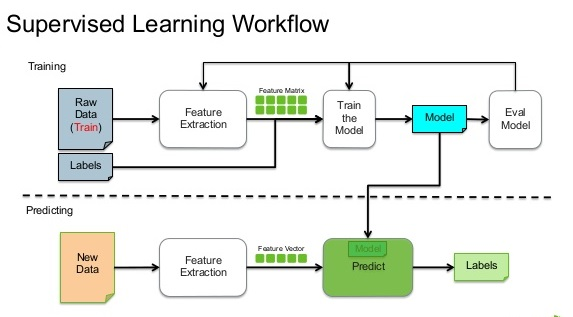
\includegraphics[scale=1.2]{chap3/image/supervise_workflow.jpeg}
\caption{Học có giám sát}
\label{fig:supervisedlearning}
\end{center}
\end{figure}
\end{center}

\end{itemize}

%\subsection{Các khái niệm cơ bản}
%\begin{itemize}
%	\item \textbf{Quan sát}: kí hiệu là \textbf{x}, input trong các bài toán. Quan sát thường có dạng là một vector $\textbf{x}=(x_1,x_2,x_3,\ldots, x_n)$, gọi là \textbf{feature vector}. Mỗi $x_i$ gọi là một feature. Ví dụ bạn muốn đoán xem hôm nay có mưa không dựa vào observation gồm các feature (nhiệt độ, độ ẩm, tốc độ gió).	
%\item \textbf{Label}: kí hiệu là $y$, output của bài toán. Mỗi quan sát sẽ có một label tương ứng. Ở ví dụ về mưa ở trên label chỉ là "mưa" hoặc "không mưa"; hay về điểm thì là các số thực từ 0 đến 10. Label có thể mang nhiều dạng nhưng đều có thể chuyển đổi thành một số thực hoặc một vector. 
%\item \textbf{Model}: trong chương này các bạn hiểu là nó là một hàm số $f(x)$, nhận vào một đầu vào \textbf{x} và trả về một đầu ra dự đoán (predict) $y=f(\textbf{x})$.
%\item \textbf{Parameter}: mọi thứ của model được sử dụng để tính toán ra output. Ví dụ model là một hàm đa thức bậc hai: $f(x) = ax_1^2 + bx_2 + c$ thì parameter của nó là bộ ba $(a,b,c)$. Để ngắn gọn, người ta thường gom tất cả parameter của một model lại thành một vector, thường được kí hiệu là $\textbf{w}$ và biểu diễn thông qua hàm $f(\textbf{x},\textbf{w}) = \textbf{x}\textbf{w}$.
%
%\end{itemize}
%\subsection{Huấn luyện mạng}
% Một mạng nơron được huyấn luyện sao cho với một tập các vector đầu vào
%X, mạng có khả năng tạo ra tập các vector đầu ra mong muốn Y của nó. Tập \textbf{X} được sử dụng cho huấn luyện mạng được gọi là tập huấn luyện (training set). Các phần tử \textbf{x} thuộc \textbf{X} được gọi là các mẫu huấn luyện (training example). Quá trình huấn luyện bản chất là sự thay đổi các trọng số liên kết của mạng. Trong quá trình này, các trọng số của mạng sẽ hội tụ dần tới các giá trị sao cho với mỗi vector đầu vào \textbf{x} từ tập huấn luyện, mạng sẽ cho ra vector đầu ra y như mong muốn.\par
%Có hai phương pháp học phổ biến là học có giám sát (supervised learning), học không giám sát (unsupervised learning):
%
%\begin{itemize}
%	\item \textbf{Học có giám sát}: Là quá trình học có sự tham gia giám sát của một "thầy giáo". Giống như ta dạy trẻ nhận diện các loại phương tiện. Ta đưa ra hình ô tô và bảo với trẻ đó rằng đây là chiếc ô tô. Việc này được thực hiện trên các loại phương tiện khác nhau như xe máy, máy bay, xe đạp.... Sau đó khi kiểm tra ta sẽ đưa ra một hình phương tiện bất kì, các hình này hơi khác so với các hình đã dạy trẻ, và cho trẻ đoán xem xe này thuộc loại phương tiện nào?\\
%	Như vậy với học có giám sát, số lớp cần phân loại đã được biết trước. Nhiệm vụ của thuật toán là phải xác định được một cách thức phân lớp sao cho với mỗi vector đầu vào sẽ được phân loại chính xác vào lớp của nó
%	
%	\item \textbf{Học không giám sát}: Là việc học không cần có bất kỳ một sự giám sát nào.Trong bài toán học không giám sát, chúng ta không biết câu trả lời chính xác cho mỗi dữ liệu đầu vào. Nhiệm vụ của thuật toán là phải phân chia tập dữ liệu đầu vào thành các nhóm con, mỗi nhóm chứa các đặc trưng giống nhau. Ví dụ như phân nhóm loại khách hàng dựa trên hành vi mua hàng: số lượng hàng hóa mua, loại hàng hóa mua, khoảng thời gian cách nhau giữa mỗi lần mua,....\\
%	 Như vậy với học không giám sát, số lớp phân loại chưa được biết trước, và tùy theo tiêu chuẩn đánh giá độ tương tự giữa các mẫu mà ta có thể có các lớp phân loại khác nhau.
%
%\end{itemize}
%Tài liệu này tôi sẽ trình bày về phần học có giám sát thông qua mạng nơ-ron nhân tạo và mạng tích chập.
%


\section{Cấu tạo của nơ-ron}
\subsection{Nơ-ron sinh học}
Cách thức hoạt động của bộ não nói riêng và của hệ thần kinh nói chung đã được con người quân tâm nghiên cứu từ rất lâu nhưng cho đến nay các nhà khoa học vẫm chưa thực sự hiểu rõ chi tiết về hoạt động của bộ não và hệ thần kinh. Đặc biệt là trong các hoạt động liên quan đến trí óc như suy nghĩ, học tập, tư duy, trí nhớ, sáng tạo....Tuy nhiên, các nhà khoa học cũng có một số thông tin căn bản về bộ não con người. Theo đó, một bộ não con người trung bình cân nặng khoảng 1,5kg và có thể tích là 235 $cm^{3}$ , cấu tạo bộ não được chia ra làm nhiều vùng khác nhau, mỗi vùng kiểm soát một hay nhiều hoạt động của con người. Hoạt động của cả hệ thống thần kinh bao gồm não bộ và các giác quan như sau: đầu tiên con người nhận được kích thích bởi các giác quan từ bên ngoài hoặc trong cơ thể. Các kích thích này được biến thành các xung điện bởi chính các giác quan tiếp nhận kích thích. Những tín hiệu này được chuyển về trung ương thần kinh là bộ não để xử lý. Tại bộ não các thông tin sẽ được xử lý, đánh giá và so sánh với các thông tin đã được lưu trữ để đưa ra các quyết định dưới dạng các xung điện. Từ những quyết định từ bộ não sẽ sinh ra các mệnh lệnh cần thiết và gửi đến những bộ phận thi hành thích hợp như các cơ tay, chân, giác quan….
\begin{center}
\begin{figure}[H]
\begin{center}
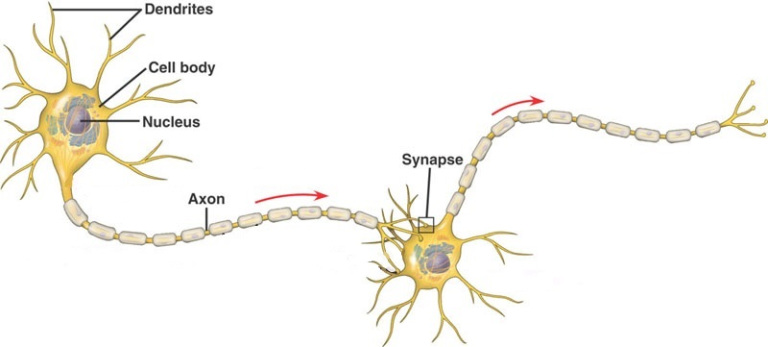
\includegraphics[scale=0.7]{chap3/image/neoronsinhhoc.jpg}
\caption{Minh họa cấu tạo nơ-ron sinh học}
\label{fig:noronsinhhoc}
\end{center}
\end{figure}
\end{center}
Khi xem xét ở mức độ tế bào thì bộ não được hình thành từ $10^11$ phần tử gọi là nơ-ron (hay neural sinh học). Mỗi neural được liên kết chặt chẽ với $10^{4}$ neural khác. Các neural này có nhiều đặc điểm chung với các tế bào khác trong cơ thể, ngoài ra chúng có những khả năng mà các tế bào khác không có được đó là khả năng nhận, xử lý và truyền các tín hiệu điện hóa làm cơ sở hình cách thức xử lý thông tin của bộ não. Hình \ref{fig:noronsinhhoc} mô tả cấu tạo và cách thức hoạt động của neural sinh học, trong đó mỗi nơ-ron sinh học có 4 thành phần cơ bản: 
\begin{itemize}
\item[-]Các nhánh tín hiệu vào (denrites) đây chính là các mạng dạng cây của các dây thần kinh truyền tín hiệu vào đến thân nơ-ron.
\item[-] Thân nơ-ron (cell body) chứa nhân (nucleus) hay một số tài liệu gọi là soma có nhiệm vụ chính là tổng hợp và xử lý các tín hiệu điện nhận vào từ các đầu vào. Bản chất của quá trình này chính là việc lấy tổng tất cả các tín hiệu neural nhận được.

\item[-]Sợi trục ra (axon) có chức năng truyền tín hiệu từ thân tế bào này sang nơ-ron khác. Phần cuối của axon được chia thành nhiều nhánh nhỏ (cả của denrites và axon) kết thúc tại khớp nối (Synapse).
\item[-]Khớp nối (Synapse) là điểm liên kết giữa sợi trục ra của nơ-ron này với các nhánh denrites của neural khác. Liên kết giữa các nơ-ron và độ nhạy của mỗi synapse được xác định bởi quá trình học phức tạp. Khi điện thế của synapses tăng lên do xung điện phát ra từ axon thì synapses sẽ tiết ra một loại hóa chất để kết nối mở ra cho các ion đi qua nó. Các ion này làm thay đổi tín hiệu điện thế trên các điểm tiếp xúc tạo ra các xung điện lan truyền tới các neural khác.
\end{itemize}

\subsection{Nơ-ron nhân tạo}
\label{sec:neuralStruct}
Cũng giống như nơ-ron sinh học, nơ-ron nhân tạo cũng nhận đầu vào và thông qua quá trình xử lý đầu vào đó để thu được kết quả là đầu ra. Các nhánh tín hiệu vào sẽ được nhận từ các sợi trục ra của các nơ-ron khác tại khớp nối và chuyển thông tin vào trong nhân, nhân nơ-ron sẽ là với hàm tổng, hàm kích hoạt và sợi trục ra của nơ-ron tương đương với đầu ra. Các thành phần trên được trình bày qua Hình \ref{fig:aNeural}. 
\begin{center}
    \begin{figure}[h]
    \begin{center}
     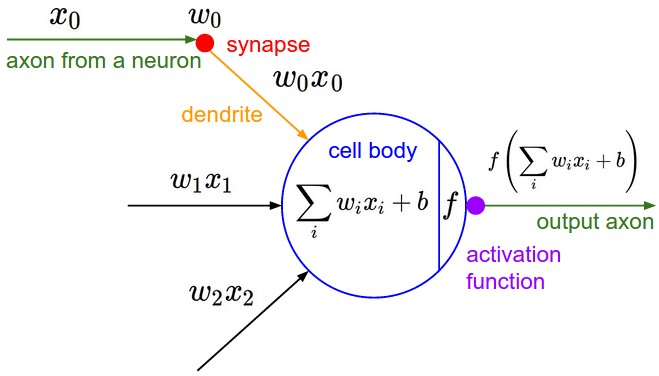
\includegraphics[scale=0.5]{chap3/image/neuron.jpeg}
    \end{center}
    \caption{Cấu trúc của một nơ-ron, nguồn: https://cs231n.github.io/}
 	\label{fig:aNeural}
    \end{figure}
\end{center}

\begin{itemize}
	\item[--]\textit{Đầu vào (input)}: là các tín hiệu vào của nơ-ron, các tín hiệu này thường đưa vào dưới dạng một vector, kí hiệu là $\textbf{x}$.
	\item[--] \textit{Trọng số (weight)}: mỗi liên kết được thể hiện bởi một trọng số liên kết và thường được kí hiệu \textit{w}. Thông thường, các trọng số này được khởi tạo một cách ngẫu nhiên theo phân phối chuẩn ở thời điểm khởi tạo mạng và được cập nhật liên tục trong quá trình học mạng.

	\item[--] \textit{Ngưỡng (bias)}: là tham số nhằm tăng khả năng thích ứng của mạng nơron trong quá trình học và thường được kí hiệu là \textit{b}. Bias gần giống như trọng số, trừ một điều là nó luôn có tín hiệu vào không đổi bằng 1.
	
	\item[--] \textit{Hàm kết hợp (combination function)}: Mỗi một đơn vị trong một mạng kết hợp các giá trị đưa vào nó thông qua các liên kết với các đơn vị khác, sinh ra một giá trị gọi là $net input$. Thông thường hàm này sẽ là hàm tổng của các tích giữa trọng số với đầu vào sau đó cộng thêm bias, được biểu diễn thông qua biểu thức $z = \sum_{i=1}^n(x_iw_i) +b$.
	\item[--] \textit{Hàm kích hoạt (activiation function hoặc transfer function)}: Hàm này được dùng để giới hạn phạm vi đầu ra của mỗi nơ-ron. Nó nhận đầu vào là kết quả của hàm kết hợp và ngưỡng đã cho. Thông thường hàm kích hoạt sẽ là các hàm phi tuyến tính.
%	 Vì nếu nó là tuyến tính thì khi kết hợp với phép toán tuyến tính $\textbf{w}^{T}\textbf{x}$ thì kết quả thu được cũng sẽ là một thao tác tuyến tính dẫn tới chuyện nó trở nên vô nghĩa.
	\item[--] \textit{Đầu ra (output)}: là tín hiệu đầu ra của một nơ-ron, với mỗi nơ-ron sẽ có tối đa là một đầu ra. Nếu như nơ-ron đó ở các hidden layer (\ref{sec:layer}) thì đầu ra của nó được gọi là activation và được kí hiệu là $a$.
\end{itemize}
\par
Khi quy về toán học thì một nơ-ron sẽ được thể hiện thông qua hai hàm sau:
\begin{center}
$z = b + \sum_{i=1}^n(w_{i}x_{i})+b = b + \textbf{w}\textbf{x}$\\[5pt]
$a = f(z)$
\end{center}
  trong đó:
\begin{itemize}
\setlength{\itemindent}{5mm}
	\item[\textendash] $x_i,w_i$ là giá trị thứ $i$ của đầu vào và trọng số tương ứng
	\item[\textendash] Hàm $f$ là hàm truyền và có đầu vào là giá trị của bộ tổng $z$
	\item[\textendash] $a$ là giá trị được tính bởi hàm truyền và là đầu ra của nơ-ron
\end{itemize}
\textbf{Một số hàm kích hoạt}
\begin{enumerate}
\item
\label{sec:relu}
\textit{Hàm ReLU} (rectified linear unit function) là hàm phi tuyến tính đơn giản nhất, có công thức toán học  $f(s)=\max(0,s)$. Đồ thị hàm ReLU được thể hiện ở Hình \ref{fig:relu}
\begin{center}
 	\begin{figure}[htp]
    \begin{center}
    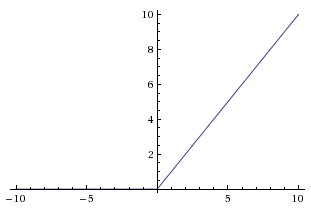
\includegraphics[scale=1]{chap3/image/relu.jpeg}
    \end{center}
    \caption{Hàm ReLU}
    \label{fig:relu}
    \end{figure}
\end{center}
Ta thấy hàm ReLU có đầu ra là 0 nếu đầu vào nhỏ hơn hoặc bằng 0, và đầu ra bằng đầu vào trong trường hợp ngược lại. Hàm ReLU có đạo hàm như sau:
	
\begin{center}
	$\frac{d}{dx}ReLU(x) =
    \begin{cases}
       0,$ if $x < 0,\\
       1,  otherwise.
    \end{cases}
    $
\end{center}
	  Hàm ReLU thường được sử dụng làm hàm truyền trong các hidden layer, còn ở layer cuối cùng thì ta sẽ sử dụng hàm khác để có thể tính toán được sắc xuất dự đoán vào vùng phân loại.

\item  \textit{Hàm sigmoid} là hàm phi tuyến tính có đồ thị một dạng đường cong hình dạng chữ "S" (Hình \ref{fig:sigmoid}) và có công thức toán học là $f(x) = \frac{1}{1+e^{x}}$. Sự tăng trưởng của đồ thị gồm giai đoạn tăng trưởng ban đầu được xấp xỉ hàm mũ và khi quá trình bão hòa bắt đầu, sự phát triển sẽ chậm lại, và tới giai đoạn trưởng thành thì dừng hẳn. \\	

\begin{center}
 	\begin{figure}[H]
    \begin{center}
    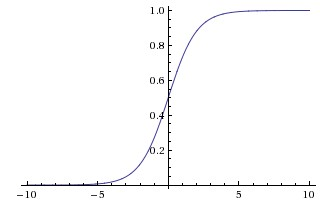
\includegraphics[scale=1]{chap3/image/sigmoid.jpeg}
    \end{center}
    \caption{Hàm sigmoid}
    \label{fig:sigmoid}
    \end{figure}
\end{center}

Giá trị của hàm số luôn nằm trong khoảng (0,1], cụ thể hơn là với đầu vào lớn hàm số sẽ cho đầu ra gần với 1 còn với đầu vào nhỏ hàm số sẽ cho đầu ra gần với 0. Đạo hàm của hàm sigmoid này khá là đẹp $f'(x) = f(x)(1-f(x))$.
%  Những năm gần đây, hàm số này ít khi được sử dụng do khi có đầu vào là những số cực lớn hoặc cực bé thì đạo hàm của hàm số xấp xỉ bằng 0, điều này gây ảnh hưởng đến việc cập nhập các trọng số trong quá trình học và làm cho thời gian tính toán lâu hơn. Tôi sẽ trình bày tại sao lại như vậy ở phần backpropagation.
	
\item
\label{sec:softmax}
\textit{Hàm softmax} hay hàm trung bình mũ là sự khái quát hóa của hàm sigmoid biến không gian K-chiều véc tơ  với giá trị thực bất kỳ đến không gian K-chiều véc tơ  mang giá trị trong phạm vi (0, 1).
Hàm softmax có phương trình toán học như sau:
\begin{center}
	$y_i=\frac{\exp({x_i})}{\sum^{n}_{j=1}{\exp({x_j})}}; \forall i=1,...,n$, \text{với $n$ là số lượng phần tử trong vector \textbf{x}}
\end{center}	
Hàm softmax có công dụng trong việc phân loại tập dữ liệu. Vì nếu tại giá trị phần tử $x_i$ lớn vượt trội so với toàn bộ dữ liệu ở vector $\textbf{x}$ thì giá trị đầu ra $y_i$ cũng sẽ lớn vượt trội so với đầu ra ở các phần tử khác. Do tổng giá trị đầu ra của hàm softmax luôn bằng môt, luôn dương và mỗi đầu ra đều phụ thuộc vào tất cả các đầu vào nên ta có thể coi giá trị đầu ra thể hiện xác suất của dữ liệu rơi vào từng tập dữ liệu tương ứng.\\
Ví dụ dữ liệu đầu vào là vector \textbf{z}, kết quả giá trị đầu ra tương ứng là vector \textbf{a} (Hình \ref{fig:vdsoftmax}). Chúng ta có thể thấy các giá trị $a_1,a_2,a_3$ thể hiện xác suất của dữ liệu $\textbf{z}$ rơi vào.
\begin{center}
	\begin{figure}[htp]
	\begin{center}
		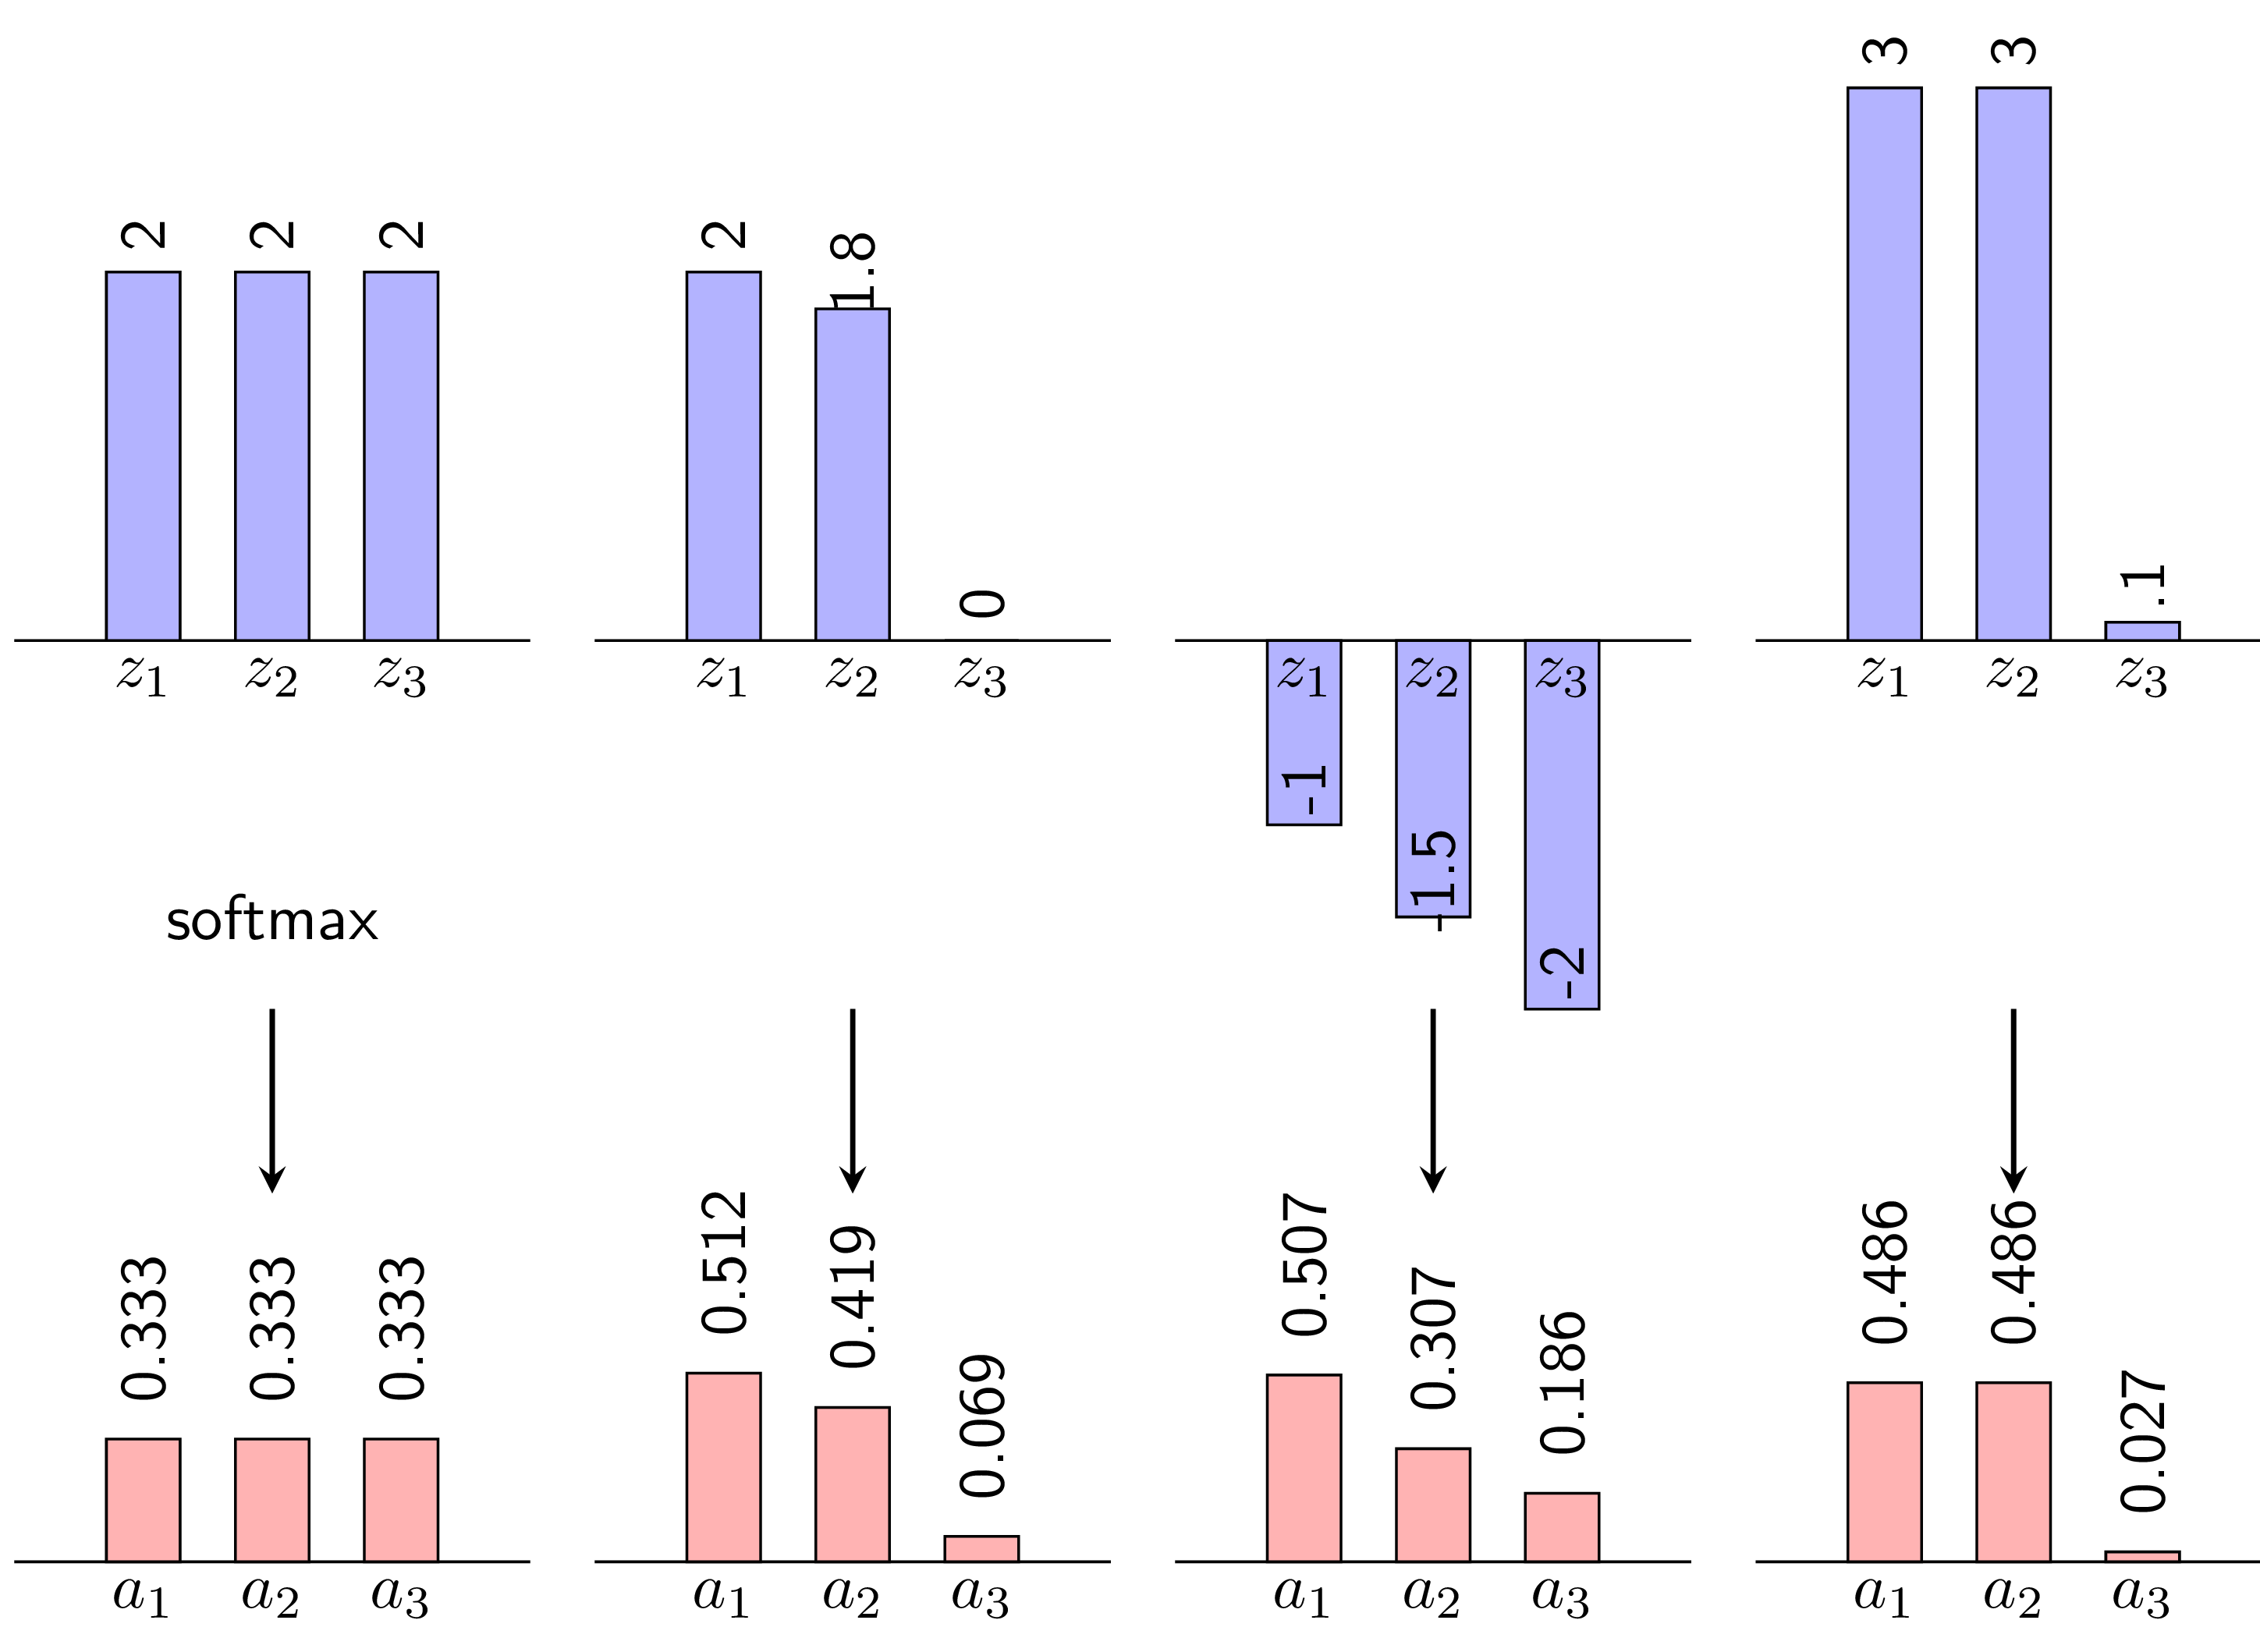
\includegraphics[scale=0.1]{chap3/image/softmax_ex.png}
	\end{center}			
	\caption{Ví dụ hàm softmax (nguồn: machinelearningcoban.com)}
	\label{fig:vdsoftmax}
	\end{figure}
\end{center}

\end{enumerate}
\section{Mạng nơ-ron nhiều lớp}
\subsection{Kiến trúc chung}
\label{sec:layer}
Mạng nơ-ron là sự kết hợp của các lớp perceptron hay còn gọi là perceptron nhiều lớp (multilayer perceptron) sẽ có nhiều lớp liên kết với nhau và được chia làm 3 lớp chính: lớp đầu vào (\textit{input layer}), lớp ẩn (\textit{hidden layer}), lớp đầu ra (\textit{output layer}). Mỗi lớp sẽ có một số lượng perceptron khác nhau, không có quy định chung và tùy theo người thiết kế mạng. Kiến trúc chung của mạng nơ-ron được minh họa trong Hình \ref{fig:neuralNetworkStruct}.
\begin{center}
 	\begin{figure}[H]
    \begin{center}
     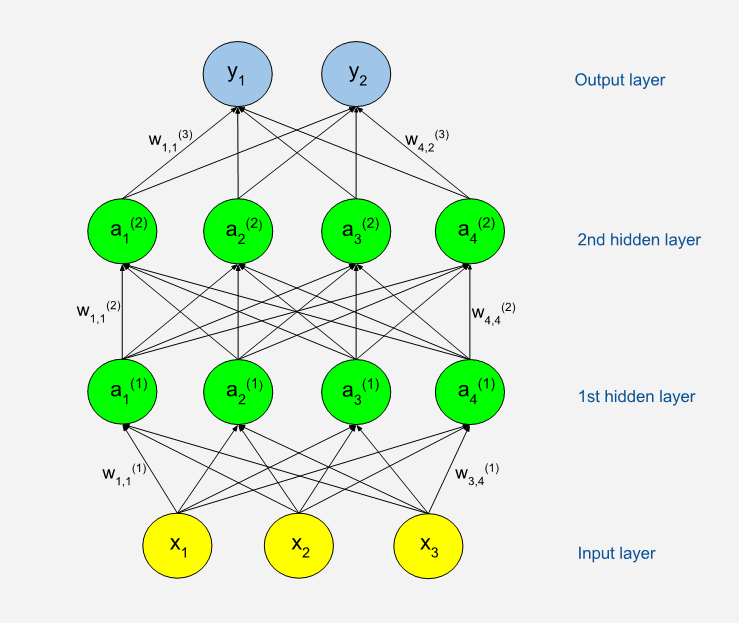
\includegraphics[scale=0.8]{chap3/image/cautrucNN.png}
    \end{center}
    \caption{Cấu trúc chung của mạng nơ-ron}
    \label{fig:neuralNetworkStruct}
    \end{figure}
\end{center}

\begin{itemize}
\setlength{\itemindent}{5mm}
	\item[-] Lớp đầu vào hay còn gọi là \textit{input layer}: Biểu diễn tổng quát của mỗi quan sát
	\item[-] Lớp đầu ra hay còn gọi là \textit{output layer}: Thể hiện đầu ra dự đoán của model
	\item[-] Lớp ẩn hay còn gọi là \textit{hidden layer}: Là lớp thể hiện cấu trúc, suy luận logic của mạng nơ-ron. Hidden layer là các lớp nằm giữa lớp đầu ra và lớp đầu vào.\end{itemize}\par
Số lượng layer trong một mạng nơ-ron được ký hiệu là $l$ và được tính bằng số hidden layer cộng thêm một, ví như mạng nơ-ron trong Hình \ref{fig:neuralNetworkStruct} là 3. Người ta gọi mỗi một nơ-ron trong mạng là một \textit{unit}.
%\subsubsection{Units}
%Mỗi \textit{node} hình trong trong Hình \ref{fig:neuralNetworkStruct} được gọi là một \textit{unit} hoặc một nơ-ron. Như tôi đã trình bày cấu trúc của một nơ-ron ở phần \ref{sec:neuralStruct}, đầu vào của một nơ-ron là một hàm kết hợp và đầu ra thông qua một hàm gọi là activiation. Ở mạng nơ-ron thì đầu vào của hidden layer thứ $l$ được ký hiệu là $\textbf{z}^{(l)}$ với $z^{(l)}_i = \textbf{x}\textbf{w}^{(l)}_i$ và đầu ra của mỗi unit được ký hiệu là $\textbf{a}^{(l)}$ với $\textbf{a}^{(l)}= f(\textbf{z}^{(l)})$.\par
%
%	Số lượng unit trong mỗi lớp, số lượng lớp trong mỗi cấu trúc mạng là không xác định. Nó được xây dựng dựa vào kinh nghiệm của người thiết kế mạng hoặc theo các tài liệu đã được công bố. Nếu số lượng lớp quá lớn thì tốc độ tính toán chậm, còn số lượng lớp ít thì độ tin cậy của kết quả không cao. Nếu số node trong các lớp lớn thì sẽ bị overfitting, ngược lại sẽ bị underfitting. Tôi sẽ trình bày phần overfitting, underfitting ở phần sau.
\subsection{Mạng lan truyền thẳng}
\subsubsection{Mô tả}
Một mạng lan truyền thẳng (\textit{feed forward}) nhiều lớp bao gồm một lớp vào, một lớp ra và một hoặc nhiều lớp ẩn. Các nơron đầu vào thực chất không phải các nơron theo đúng nghĩa, bởi lẽ chúng không thực hiện bất kỳ một tính toán nào trên dữ liệu vào, đơn giản nó chỉ tiếp nhận các dữ liệu vào và chuyển cho các lớp kế tiếp. Các nơron ở lớp ẩn và lớp ra mới thực sự thực hiện các tính toán, kết quả được định dạng bởi hàm đầu ra. Cụm từ “truyền thẳng” (feed forward) (không phải là trái nghĩa của lan truyền ngược) liên quan đến một thực tế là tất cả các nơ-ron chỉ có thể được kết nối với nhau theo một hướng: tới một hay nhiều các nơron khác trong lớp kế tiếp (loại trừ các nơron ở lớp ra). Cụ thể hơn là không có các liên kết từ các nơ-ron ở lớp đầu ra đến các nơ-ron ở các lớp đầu và hay các nơ-ron trong cùng một lớp cũng không có liên kết với nhau. Các lớp lớp liên kết với nhau theo quy luật đầu vào lớp sau là đầu ra của lớp trước.
\subsubsection{ Thuật toán}
\label{subsec:feedforward}

\begin{algorithm}[H]
\caption{Forward propagation }\label{al:forward}
\begin{algorithmic}
\REQUIRE Network depth, $l$
\REQUIRE $\textbf{W}^{(i)}, i \in \{1,\ldots,l\}$, ma trận trọng số của model
\REQUIRE $\textbf{b}^{(i)}, i\in \{1,\ldots,l\}$tham số bias của model
\REQUIRE $\textbf{X}, \textbf{x}_i, i \in \{1,\ldots,N\} $, tập dữ liệu đầu vào với $N$ là số lượng dữ liệu.
\FOR {$j=1,\ldots,N$}
	
	\STATE $\textbf{a}^{(0)} = \textbf{x}_j$
	\FOR {$i=1,\ldots,l$}
		\STATE $\textbf{z}^{(i)}= \textbf{b}^{(i)} + \textbf{W}^{(i)}\textbf{a}^{(i-1)} $
		\STATE $\textbf{a}^{(i)}=f(\textbf{z}^{(i)})$
\ENDFOR
\STATE $\widehat{\textbf{y}} = \textbf{a}^{(L)}$
\ENDFOR
\end{algorithmic}
\end{algorithm}
\subsubsection{Ví dụ}
  Giả sử ta có mạng neural như Hình \ref{fig:baitoan} với tập dữ liệu đầu vào là ma trận $\textbf{X}_{2{\times}N}$ ($N$ là số lượng quan sát, 2 là số lượng feature), và label tương ứng là vector $\textbf{y}_{N\times 1}$ (2 là số lượng nhãn), $\textbf{y}_i \in (1,2,3,\ldots,C)$ với C là số lớp cần phân loại .

\begin{figure}[H]
\begin{center}
	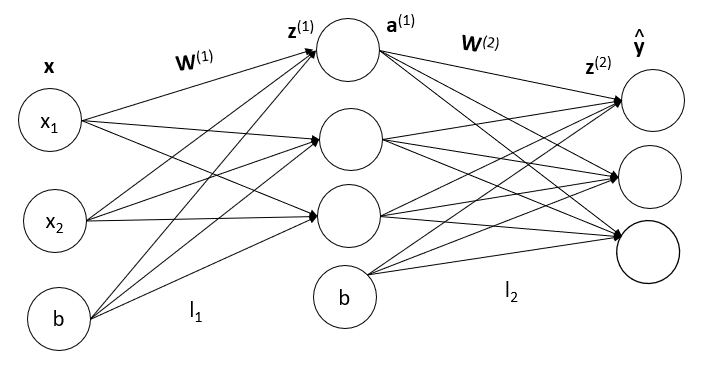
\includegraphics[scale=1]{chap3/image/myNeuralNetwork.png}
	\caption{Mạng neural cho bài toán }
	\label{fig:baitoan}
\end{center}
\end{figure}


Xét một cặp dữ liệu $(\textbf{x}_i,\textbf{y}_i)$ với hàm activation ở hidden layer là hàm relu, hàm activation ở output layer là hàm softmax. Mạng lan truyền thẳng sẽ được tính như sau:

\begin{eqnarray}
\textbf{x}_{1\times 2} &=&\begin{bmatrix} x_1 &x_2 \end{bmatrix} \textbf{W}^{(1)T}_{3{\times}2}  =\begin{bmatrix}
	w^{(1)}_{11} &w^{(1)}_{12} \\[6pt]
	w^{(1)}_{21} &w^{(1)}_{22} \\[6pt]
	w^{(1)}_{31} &w^{(1)}_{32} 
\end{bmatrix}^{T} \label{eq:s1}\\
\textbf{z}^{(1)}_{1 \times 3} &=&	\textbf{x}_{1\times 2}\textbf{W}^{(1)T}_{3\times 2} +b^{(1)}	= \begin{bmatrix}
z^{(1)}_{1} &z^{(1)}_{2} &z^{(1)}_{3} 
\end{bmatrix} \label{eq:s2}	\\
\label{eq:s3}
\textbf{a}^{(1)}_{1 \times 3}	&=&		\max(0,\textbf{z}^{(1)} =	\begin{bmatrix}
	a^{(1)}_1 &a^{(1)}_2 &a^{(1)}_3 
	\end{bmatrix}\\
\label{eq:s4}
\textbf{W}^{(2)T}_{3{\times}3}  &=&	 \begin{bmatrix}
	w^{(2)}_{11} &w^{(2)}_{11} & w^{(2)}_{13}\\[6pt]
	w^{(2)}_{21} &w^{(2)}_{22} & w^{(2)}_{23}\\[6pt]
	w^{(2)}_{31} &w^{(2)}_{32} & w^{(2)}_{33}
\end{bmatrix}^T  \\
\label{eq:s5}
\textbf{z}^{(2)}_{1\times 3}	&=&\textbf{a}^{(1)}_{1 \times 3}\textbf{W}^{(2)T}_{3{{\times}}3}+b^{(2)}	= \begin{bmatrix}
z^{(2)}_{1} &z^{(2)}_{2} &z^{(2)}_{3} 
\end{bmatrix}\\
\label{eq:s6}
\widehat{\textbf{y}}&=&\textbf{a}^{(2)}_{1\times 3} 	= \frac{\exp({\textbf{z}^{(2)}})}{\sum^{2}_{j=1}{\exp({\textbf{z}^{(3)}_j})}}
\end{eqnarray}


Tại các biểu thức số \ref{eq:s1},\ref{eq:s4} là giá trị đầu vào và khởi tạo ma trận trọng số cho layer thứ 1,2; tại biểu thức số \ref{eq:s2},\ref{eq:s5} ta tính giá trị hàm kết hợp (bộ tổng) làm input đầu vào cho nơ-ron; tại biểu thức số \ref{eq:s3},\ref{eq:s6} ta tính đầu ra cho mỗi nơ-ron. Ở layer thứ nhất đầu ra nơ-ron sử dụng \textit{hàm ReLU} \ref{fig:relu} làm hàm activation vì thế tại biểu thứ số \ref{eq:s3} ta có  $\textbf{a}^{(1)}_{1 \times 3}	=\max(0,\textbf{z}^{(1)})$ còn tại layer thứ hai sử dụng hàm softmax làm hàm đầu ra cho nơ-ron nên ta có $\textbf{a}^{(2)}_{1\times 3} = \frac{\exp({\textbf{z}^{(2)}})}{\sum^{3}_{j=1}{\exp({\textbf{z}^{(2)}_j})}}$.


Với tập dữ liệu $(\textbf{X},\textbf{y} )$ thì ta có đầu ra dự đoán như sau:  
\begin{center}

	$\widehat{\textbf{Y}} =\frac{\exp({\textbf{z}^{(2)}_i})}{\sum^{2}_{j=1}{\exp({\textbf{z}^{(2)}_{ij}})}}$; với $i=1,2,...,N$ 

\end{center}
Việc tính toán tuần tự như vậy được được gọi là \textit{feedforward}.
\subsection{Hàm mất mát}
  Hàm mất mát hay còn gọi là \textit{loss function} hoặc \textit{cost function}, là sự chêch lệch, khác biệt giữa đầu ra dự đoán và đầu ra thực tế bằng một số thực không âm, có chức năng là đo độ chính xác của đầu ra dự đoán, thường được ký hiệu là $J$. Ví dụ ta cần ánh xạ: $\textbf{x}\to \textbf{y}$,  trong đó $\textbf{x}$ là tập các dữ liệu và $\textbf{y}$ là tập các nhãn tương ứng cho từng dữ liệu thì ta cần \textit{ước lượng các tham số} $\textbf{w}$ sao cho thỏa mãn $ f(\textbf{x},\textbf{w}) \approx \textbf{y}$, giá trị của hàm $f$ được kí hiệu là $\widehat{\textbf{y}}$. Khi đó hàm mất mát là độ chênh lệch, sự khác biệt giữa \textbf{$\widehat{\textbf{y}}$} và $\textbf{y}$. Nếu như giá trị mất mát càng lớn thì điều đó có nghĩa rằng đầu ra dự đoán càng sai, các tham số truyền vào chưa chính xác vì thế chúng ta cần điều chỉnh lại các tham số sao cho tập giá trị của \textbf{$\widehat{\textbf{y}}$} càng gần $\textbf{y}$ càng tốt. Có nghĩa rằng ta cần tìm $\textbf{w}$ sao cho giá trị mất mát là nhỏ nhất: $\textbf{w}$=$\arg\min_{\textbf{w}} J $ hay nói cách khác là tìm $\textbf{w}$ sao cho tỉ lệ rơi vào đúng tập nhãn là cao nhất: $\textbf{w}$=$\arg\max_{\textbf{w}} p(\textbf{y}|\textbf{x},\textbf{w})$. Có nhiều hàm có thể làm hàm mất mát như: sai số bình phương trung bình, perceptron, hinge,cross-entropy,...
  
\subsubsection{Hàm sai số bình phương trung bình}
Hàm sai số toàn phương trung bình hay mean squared error (MSE), là hàm tiếp cận dễ nhất để hiểu hàm mất mát. Nó được định nghĩa là trung bình của bình phương các sai số giữa giá trị ước lượng được và thực tế.\par
Giả sử $\widehat{\textbf{y}}$ là một vector đầu ra dự đoán, và $\textbf{y}$ là vector đầu ra thực tế quan sát được, tương ứng với các dữ liệu đầu vào, thì MSE của phép dự báo có thể ước lượng theo công thức:
\begin{align*}
MSE = 
\frac{1}{n}
\sum_{i=1}^{n} (\textbf{y}_i - \widehat{\textbf{y}})^{2}
\end{align*}

\subsubsection{Hàm cross-entropy}
\begin{enumerate}
\item  \textit{Cross entropy}\\
Cross entropy được dùng để đo sự giống nhau của hai phân phối xác suất, giá trị của hàm số càng nhỏ thì hai xác suất càng gần nhau. Cho một phân bố xác suất $\textbf{p} = [p_1, p_2,\dots, p_n]$ với $q_i \in [0,1]$ và $\sum_{i=1}^{n} q_i = 1$. Nếu ta có một phân bố xác suất bất kỳ $\textbf{q} = [q_1, q_2, \dots, q_n]$ và $q_i \neq 0, \forall i$ thì hàm số cross entropy giữa hai phân bố $\textbf{p}$ và $\textbf{q}$ được định nghĩa là:
\begin{equation}
\label{eqn:cross2}
H(\textbf{p}, \textbf{q}) =-\sum_{i=1}^C p_i \log q_i 
\end{equation}\par

\textbf{Chú ý}: Hàm cross entropy không có tính đối xứng $H(\textbf{p}, \textbf{q}) \neq H(\textbf{q}, \textbf{p})$. Theo công thức \ref{eqn:cross2} chúng ta có thể thấy giá trị của $\textbf{q}$ không thể nhận giá trị là 0. Vì thể khi sử dụng cross entropy trong các bài toán học có giám sát, chúng ta phải để $\textbf{p}$ là đầu ra thực tế vì chỉ có vị trí nhãn là được đánh dấu 1, các vị trí còn lại được đánh dấu 0 (sử dụng one-hot encoding), $\textbf{q}$ là đầu ra dự đoán vì không có xác suất nào bằng 0 tuyệt đối.


%\subsubsection{Xây dựng hàm mất mát}
%\label{subsec:cossfunction}
%  Giả sử chúng ta tập dữ liệu $(\textbf{x}_i,y_i), ~ i = 1,2, \ldots,N$ và cần phân loại ra $C$ lớp. Xét một cặp dữ liệu $(\textbf{x}_i,\textbf{y}_i)$ với $\textbf{y}_i$ là đầu ra thực tế ở  dạng onehot vector. Chúng ta thực hiện lan truyền thẳng với mô hình có $l$ layer và hàm activation ở layer cuối là hàm softmax (refer), $\widehat{\textbf{y}_i} = softmax(\textbf{z}^{(l)})$. Có thể thấy rằng giá trị $\widehat{\textbf{y}_{ij}}$\textit{ với j=1,...,C} thể hiện xác suất để $\textbf{x}_i$ rơi vào lớp thứ $j$ và nếu coi  hai vector $\widehat{\textbf{y}_{i}}$, $\textbf{y}_i$ lần lượt tương ứng với $\textbf{q},\textbf{p}$ trong biểu thức \ref{eqn:cross2} thì \textit{giá trị mất mát} được tính như sau:
\item \textit{One-hot encoding}\\
One-hot encoding là mã hóa dữ liệu thành các vector ở dạng phân loại tức là chỉ có duy nhất một phần tử bằng 1 còn các phần tử khác bằng 0. Ví dụ ta có tập dữ liệu $y=[1,2,4,1,1]$ và cần phân loại ra 4 lớp là 1, 2, 3, 4, khi đó mã hóa các dữ liệu về dạng one-hot ta thu được tập dữ liệu tương ứng $y=[1000,0100,0001,1000,1000]$.

\item \textit{Ví dụ}\\
Tại đây tôi sẽ tiếp tục với ví dụ ở phần mạng lan truyền thẳng, các đầu ra đều được chuyển về dạng one-hot và lấy hàm cross-entropy làm hàm mất mát. Ta viết được hàm mất mát cho dữ liệu thứ $i$ như sau:
\begin{equation*}
\begin{split}
J_i(\textbf{x}_i,\textbf{y}_i)=J_i &=-\sum_{j=1}^C y_{ij} \log \widehat{y}_{ij}	\\
&= -\sum_{j = 1}^C y_{ij}\log\frac{e^{z^{(l)}_{ij}}}{\sum_{k=1}^C e^{z^{(l)}_{ik}}}\\
&= -\sum_{j=1}^C\left(y_{ij} z^{(l)}_{ij}-\log(\sum_{k=1}^C e^{z^{(l)}_{ik}})\right) \\
&= -\sum_{j=1}^C y_{ij} z^{(l)}_{ij} + \sum_{j=1}^C y_{ji}\log(\sum_{k=1}^C e^{z^{(l)}_{ik}}) 
\end{split}
\end{equation*}
vì đầu ra thực tế ở dạng onehot nên ta có  $\sum_{j=1}^C y_{ij = 1}$ mà $\log(\sum_{k=1}^C e^{z^{(l)}_{ik}})$ là hằng số nên ta có $ \sum_{j=1}^C y_{ji}\log(\sum_{k=1}^C e^{z^{(l)}_{ik}}) = \log(\sum_{k=1}^C e^{z^{(l)}_{ik}})$. Hàm mất mát được rút gọn lại như sau:
\begin{align}
\label{eq:cost1}
J_i(\textbf{x}_i,\textbf{y}_i) = -\sum_{j=1}^C y_{ij} z^{(l)}_{ij} +\log(\sum_{k=1}^C e^{z^{(l)}_{ik}})
\end{align}
\par

Như vậy đốivới tập dữ liệu $(\textbf{x}_i,y_i)$, $i=1,2,...,N$ thì hàm mất mát cho \textit{softmax} được tính theo biểu thức sau đây:
\begin{equation}
\label{eq:cost2}
J(\textbf{X},\textbf{Y})
= -\frac{1}{N}\sum_{i=1}^{N}\sum_{j=1}^C y_{ij} \log \widehat{y}_{ij}
=-\frac{1}{N} \sum_{i=1}^N \left(  \sum_{j=1}^C y_{ij}z^{(l)}_{ij} + \log\sum_{k=1}^C (e^{z^{(l)}_{ik}}) \right)
\end{equation} 
\end{enumerate}

\subsection{Thuật toán lan truyền ngược và cập nhật tham số}
Trong tiếng Anh, Lan truyền ngược là Backpropagation, là một từ viết tắt cho "backward propagation of errors" tức là "truyền ngược của sai số", là một phương pháp phổ biến để huấn luyện các mạng thần kinh nhân tạo được sử dụng kết hợp với một phương pháp tối ưu hóa như gradient descent. Phương pháp này tính toán gradient của hàm tổn thất với tất cả các trọng số có liên quan trong mạng nơ ron đó. Gradient này được đưa vào phương pháp tối ưu hóa, sử dụng nó để cập nhật các trọng số, để cực tiểu hóa hàm tổn thất.

\subsubsection{Mô tả thuật toán}
Truyền ngược yêu cầu một đầu ra mong muốn, đã biết cho mỗi giá trị đầu vào để tính toán gradient hàm tổn thất. Do đó, nó thường được xem là một phương pháp học có giám sát, tuy nhiên nó cũng được sử dụng trong một số mạng không có giám sát. Nó là tổng quát hóa của gradient descent cho các mạng lan truyền thẳng nhiều lớp, thực hiện bằng cách sử dụng quy tắc chain rule để tính toán lặp đi lặp lại các gradient cho mỗi lớp. Thuật toán lan truyền ngược yêu cầu các hàm kích hoạt được sử dụng bởi các nơ-ron nhân tạo khả vi.
\subsubsection{Thuật toán}

\begin{algorithm}[H]
\caption{Backpropagation }\label{al:forward}
\begin{algorithmic}
\REQUIRE Network depth, $l$
\REQUIRE $\textbf{W}^{(i)}, i \in \{1,\ldots,l\}$, ma trận trọng số của model
\REQUIRE $\textbf{b}^{(i)}, i\in \{1,\ldots,l\}$tham số bias của model
\REQUIRE $ \textbf{x}_i, i \in \{1,\ldots,N\} $, tập dữ liệu đầu vào
\REQUIRE $\textbf{y}_i,i \in \{1,\ldots,N\} $, đầu ra thực tế
\REQUIRE ${\widehat{\textbf{y}}}$, đầu ra dự đoán
\REQUIRE $\textbf{z},\textbf{a}$, đầu ra của hàm kết hợp và hàm kích hoạt
\REQUIRE $J$, giá trị của hàm mất mát
\STATE Sau khi thực hiện thuật toán lan truyền thẳng, tính gradient ở lớp đầu ra:
\STATE $\textbf{g} \gets \frac{\partial J}{\partial\widehat{y}} $
\FOR {$k=1,\ldots,l$}	
	\STATE Từ lớp đầu ra, tính gradient quay lui với hàm kích hoạt ở lớp thứ $k$ theo chain rule
	\STATE $\textbf{g} \gets \frac{\partial J}{\partial \textbf{z}^{(k)}} = \textbf{g} \odot f'(\textbf{z}^{(k)})$
	\STATE Tính gradient so với trọng số, ngưỡng
	\STATE $\frac{\partial J}{\partial \textbf{b}^{(k)}} = \textbf{g}$
	\STATE $\frac{\partial J}{\partial \textbf{W}^{(k)}} = \textbf{g}\textbf{a}^{(k-1)T}$
	\STATE Gradient được đưa xuống lớp đầu ra thấp hơn
	\STATE $\textbf{g} \gets \frac{\partial J}{\partial \textbf{a}^{(k-1)}} = \textbf{W}^{(k)T}\textbf{g} $
\ENDFOR
\end{algorithmic}
\end{algorithm}

\subsubsection{Ví dụ}
  Ta sử dụng mạng nơ-ron ở Hình \ref{fig:baitoan}, xét một cặp dữ liệu thứ $i$ ta có $(\textbf{x}_i,\textbf{y}_i)$ với $\textbf{x}_{i}$ là đầu vào và $\textbf{y}_i$ là đầu ra thực tế ở dạng \textit{one-hot}. Để thực hiện được thuật toán chúng ta cần tìm đầu ra dự đoán thông qua lan truyền thẳng (refer), tính giá trị mất mát (refer). Tôi xin được viết lại như sau:
\begin{itemize}
	\item[] $\textbf{a}^{(0)}_{i}=\textbf{x}_{i}$
	\item[]  $\textbf{z}^{(1)}_{i}= \textbf{b}^{(1)} + \textbf{W}^{(1)}\textbf{a}^{(0)}_{i}$
	\item[] $\textbf{a}^{(1)}_{i}=\max(0,\textbf{z}^{(1)}_{i})$
	\item[] $\textbf{z}^{(2)}_{i}=\textbf{b}^{(2)} + \textbf{W}^{(2)}\textbf{a}^{(1)}_{i}$	
	\item[] $ \textbf{a}^{(2)}_{i} = \widehat{\textbf{y}}_{i} = softmax(\textbf{z}^{(2)}_i) = \frac{\exp({\textbf{z}^{(2)}_i})}{\sum^{3}_{j=1}{\exp({\textbf{z}^{(2)}_j})}}$
\end{itemize}
và hàm mất mát: $J_i = - \sum_{j=1}^{3}y_{ij}\log\widehat{y}_{ij} $\\
Vì chỉ xét trên một cặp dữ liệu và để dễ nhìn hơn, ta lược bỏ chỉ số $i$ ở các biểu thức tính toán dưới đây. Theo như thuật toán lan truyền ngược, trước tiên ta cần tính đạo hàm của đầu ra dự đoán đối với hàm mất mát. Xét đầu ra dự đoán thứ $k$ của tập dữ liệu thứ $i$.
\begin{equation*}
\begin{split}
g^{(l)}_k & = \frac{\partial J}{\partial \widehat{y}_k}
= -\sum_{j=1}^{3} y_j \frac{\partial \log\widehat{y}_{j}}{\widehat{y}_{k}}
= -\sum_{j=1}^{3} y_j \frac{1}{\widehat{y}_k}
\end{split}
\end{equation*}
Tiếp theo ta đưa đạo hàm về layer cuối cùng, tương đương với $l=2$, ta có $\textbf{g}^{(l)} = \textbf{g}^{(l)} \odot f'(\textbf{a}^{(l)})$, với hàm $f(\textbf{z}^{(2)})$ là hàm softmax. Để biểu thức sau này của chúng ta bớt cồng kềnh, tôi sẽ tính riêng đạo hàm của hàm softmax. Đối với hàm này chúng ta cần lưu ý rằng nó có hai trường hợp là đạo hàm phần tử trùng với tử số hoặc khác tử số.\\
Giả sử hàm softmax chúng ta có như sau: $p_i = \frac{e^{a_i}}{\sum_{k=1}^N e^{a_k}}$ và ta cần tính đạo hàm của $p_i$ đối với $a_j$ bất kì, tương đương với biểu thức $\frac{\partial p_i}{\partial a_j} = \frac{\partial \frac{e^{a_i}}{\sum_{k=1}^N e^{a_k}}}{\partial a_j}$ \\
Với $i=j$,
\begin{equation}
\label{eqn:softmaxderivative1}
\begin{split}
\frac{\partial  \frac{e^{a_i}}{\sum_{k=1}^N e^{a_k}}}{\partial a_j}&= \frac{e^{a_i} \sum_{k=1}^N e^{a_k} - e^{a_j}e^{a_i}}{\left( \sum_{k=1}^N e^{a_k}\right)^2} \\
&= \frac{e^{a_i} \left( \sum_{k=1}^N e^{a_k} - e^{a_j}\right )}{\left( \sum_{k=1}^N e^{a_k}\right)^2} \\
&= \frac{ e^{a_j} }{\sum_{k=1}^N e^{a_k} } \times \frac{\left( \sum_{k=1}^N e^{a_k} - e^{a_j}\right ) }{\sum_{k=1}^N e^{a_k} } \\
&= p_i(1-p_j)
\end{split}
\end{equation}
với $i \neq j$,
\begin{equation}
\label{eqn:softmaxderivative2}
\begin{split}
\frac{\partial  \frac{e^{a_i}}{\sum_{k=1}^N e^{a_k}}}{\partial a_j}&= \frac{0 - e^{a_j}e^{a_i}}{\left( \sum_{k=1}^N e^{a_k}\right)^2} \\
&= \frac{- e^{a_j} }{\sum_{k=1}^N e^{a_k} } \times \frac{e^{a_i} }{\sum_{k=1}^N e^{a_k} } \\
&= - p_j.p_i
\end{split}
\end{equation}
Từ biểu thức \ref{eqn:softmaxderivative1} và \ref{eqn:softmaxderivative2} ta có thể viết lại đạo hàm của softmax :\\
\begin{equation}
\frac{\partial p_i}{\partial a_j} = 
\begin{cases}
p_i(1-p_j) & if ~~i=j \\
-p_j.p_i & if ~~i \neq j\
\end{cases}
\end{equation}
Từ đó ta tính được đạo hàm như sau:
\begin{equation}
\begin{split}
g^{(2)}_k 
& = - y_k \frac{1}{\widehat{y}_k} f(z_k)(1-f(z_k))- \sum^{3}_{\substack{j=1,\\j \neq k}} y_j \frac{1}{\widehat{y}_k}(-f(z_k)f(z_j))\\
& = -y_k \frac{1}{\widehat{y}_k} \widehat{y}_k (1- \widehat{y}_k )- \sum^{3}_{\substack{j=1,\\j \neq k}} y_j \frac{1}{\widehat{y}_k}(-\widehat{y}_k \widehat{y}_j) \\
& = -y_k(1- \widehat{y}_k )+\sum^{3}_{\substack{j=1,\\j \neq k}} y_j \widehat{y}_j \\
& = -y_k + y_k\widehat{y}_k +\sum^{3}_{\substack{j=1,\\j \neq k}} y_j \widehat{y}_j\\
& = \widehat{y}_k ( y_k +\sum^{3}_{\substack{j=1,\\j \neq k}}y_j ) - y_k
\end{split}
\end{equation}
Do đầu ra thực tế $\textbf{y}$ ở dạng onehot vì thế $\sum^{3}_{j=1}y_j =1$ và $y_k +\sum^{3}_{\substack{j=1,\\j \neq k}} y_j = 1$. Vì thế ta được
\begin{align*}
g^{(2)}_k=\widehat{y}_k - y_k 
\end{align*}
Nếu ta sử dụng biểu thức \ref{eq:cost1} thì đạo hàm $\frac{\partial J}{\partial z^{(l)}_k}$ đơn giản hơn khá nhiều
\begin{equation*}
\begin{split}
\frac{\partial J}{\partial z_k}  
&=\frac{-\sum_{j=1}^C y_{kj} z^{(l)}_{kj} +\log(\sum_{m=1}^C e^{z^{(l)}_{m}})}{\partial z^{(l)}_k}\\
&=-y_{k} + 
\frac{e^{(z^{(l)})}_{k}}{\sum_{m = 1}^C e^{(z^{(l)}_m)})}\\
&= -y_{k} + \widehat{y}_k =  \widehat{y}_k -y_{k}  
\end{split}
\end{equation*} 
Tổng quát hóa với cặp dữ liệu thứ $i$ ta được
\begin{align}
\textbf{g}^{(2)}_i
= \frac{\partial J}{\partial \textbf{z}^{(2)}_i}
= \widehat{\textbf{y}}_i -  \textbf{y}_i
\end{align}
Như vậy chúng ta có 
\begin{align}
\frac{\partial J}{\partial \textbf{b}^{(2)}} 
&= \textbf{g}^{(2)}_i \label{eqn:djdb2} \\ 
\frac{\partial J}{\partial \textbf{W}^{(2)}}
& = \textbf{g}^{(2)}_i \textbf{a}^{(1)T} \label{eqn:djdw2} \\
\textbf{g}^{(2)}_i &= \textbf{W}^{(1)T}\textbf{g}^{(2)}_i \label{eqn:g1}\\
\end{align}
Tiếp theo chúng ta tính đạo hàm ở layer $l-1$ tương đương với layer đầu tiên. Layer này khá là đơn giản vì hàm activation là hàm Relu và có đạo hàm là 
\begin{align*}
f'(x)=
\begin{cases} 
0 & \text{if  }  x < 0 \\
1 & \text{if  }  x > 0 \\
\end{cases}
\end{align*} 

Từ đó ta tính được 
\begin{align*}
\textbf{g}^{(1)}_i 
&= \textbf{g}_{i}^{(1)} \odot f'(\textbf{z}^{(1)})\\
\frac{\partial J}{\partial b^{(1)}} 
&= \textbf{g}^{(1)}_i\\
\frac{\partial J}{\partial \textbf{W}^{(1)}}
&= \textbf{g}^{(1)}_i\textbf{a}^{(0)}
\end{align*}



%*/
%Chúng ta có thể thấy cách tính toán trên cũng cho kết quả với kết quả tại biểu thức \ref{eq:back_gra1}, như vậy chúng ta đã có các đạo hàm $\frac{\partial J_i(\textbf{W})}{\partial \textbf{W}^{(2)}}$. Tiếp theo chúng ta sẽ tính $\frac{\partial J_i(\textbf{W})}{\partial \textbf{W}^{(1)}}$.
%\begin{eqnarray*}
%\frac{\partial J(\textbf{W})}{\partial \textbf{w}^{(1)}_j} &=& \textbf{e}^{(L)}\frac{\partial\textbf{z}^{(2)}}{\partial \textbf{a}^{(1)}} \frac{\partial \textbf{a}^{(1)}}{\partial \textbf{z}^{(1)}_j} \frac{\partial \textbf{z}^{(1)}_j}{\partial \textbf{w}^{(1)}_j}  \\
%&=&(\textbf{a}^{(2)}-\textbf{y})\times\textbf{w}^{(2)T}_j \times1\times\textbf{a}^{(0)}\\
%&=&\textbf{a}^{(0)}e^{(1)T}
%\end{eqnarray*}
%Tổng quát hóa ta có:
%\begin{equation}
%\frac{\partial J(\textbf{W})}{\partial \textbf{W}^{(1)}} = (\textbf{a}^{(2)}-\textbf{y})\textbf{W}^{(2)T} 1 \textbf{a}^{(0)} = \textbf{a}^{(0)}\textbf{e}^{(1)T}
%\end{equation}
%Như vậy với tập dữ liệu $N$ quan sát thì chúng ta có thể như sau:
%\begin{equation}
%\begin{split}
%\frac{\partial J(\textbf{W})}{\partial \textbf{W}^{(2)}} &=\sum^{N}_{i=1} \textbf{a}^{(2-1)}_i\textbf{e}^{(2)T}_i = \textbf{A}^{(2-1)}\textbf{E}^{(2)T}\\
%\frac{\partial J(\textbf{W})}{\partial \textbf{W}^{(1)}} &= \sum^{N}_{i=1} \textbf{a}^{(0)}_i \textbf{e}^{(1)T}_i = \textbf{X}\textbf{E}^{(1)T}
%\end{split}
%\end{equation}
%với $\textbf{E}^{(2)} = \textbf{A}^{(2)}-\textbf{Y}, ~ \textbf{E}^{(1)} = \textbf{E}^{(2)}\textbf{W}^{(2)T}$
%Bước tiếp theo là sử dụng kết quả vừa tìm được để tối ưu hàm mất mát bằng các phương pháp tối ưu tôi đã trình bày ở phần \ref{sec:toiuu}. Ví dụ tôi chọn phương pháp gradient descent, chúng ta có:
%\begin{equation}
%\begin{split}
%\textbf{E}^{(2)} &= \textbf{A}^{(2)}-\textbf{Y}\\
%\textbf{W}^{(2)} &=\textbf{W}^{(2)} + \eta \textbf{A}^{(2-1)}\textbf{E}^{(2)T} \\
% \textbf{E}^{(1)} &= \textbf{E}^{(2)}\textbf{W}^{(2)T}\\
%\textbf{W}^{(1)} &= \textbf{W}^{(1)} + \eta \textbf{X}\textbf{E}^{(1)T}\\
%\end{split}
%\end{equation}
\subsection{Overfitting}
\subsubsection{Khái niệm}
  Overfitting là một hiệnn tượng không mong muốn thường gặp trong quá trình xây dựng mô hình, người xây dựng mô hình cần nắm được một số kỹ thuật để giải quyết khi vấn đề này xảy ra. Trước tiên chúng ta cần biết ba khái niệm dưới đây:
\begin{itemize}
\item []
\textit{\textbf{Underfitting}} là hiện tượng mô hình chưa được phù hợp với tập dữ liệu huấn luyện và cả các mẫu mới khi dự đoán. Nguyên nhân có thể là do mô hình chưa đủ độ phức tạp cần thiết để bao quát được tập dữ liệu.
\item []
\textit{\textbf{Overfitting}} là hiện tượng mô hình quá khớp với \textit{tập dữ liệu huấn luyện (training set)}, việc này sẽ gây ra hậu quả vô cùng nghiêm trọng nếu tập dữ liệu huấn luyện xuất hiện nhiễu. Mô hình sẽ chỉ chú trọng vào việc xấp xỉ với tập dữ liệu huấn luyện mà quên đi mục đích ban đầu là tổng quát hóa, làm cho mô hình sẽ không thật sự tốt dối với dữ liệu nằm ngoài dữ liệu huấn luyện (dữ liệu test và dữ liệu thực tế). Overfitting xảy ra khi \textit{độ phức tạp của mô hình quá lớn} hoặc \textit{quá ít dữ liệu}.
\item []
\textit{\textbf{Good fitting}} là mô hình nằm giữa 2 mô hình chưa khớp (\textit{underfitting}) và quá khớp (\textit{overfitting}) cho ra kết quả hợp lý với cả tập dữ liệu huấn luyện và các giá trị mới, tức là nó mang được tính tổng quát như hình 1 ở giữa phía trên. Lý tưởng nhất là khớp được với nhiều dữ liệu mẫu và cả các dữ liệu mới. Tuy nhiên trên thực tế được mô hình như vậy rất hiếm.
\end{itemize}
  Để hiểu vấn đề này chúng ta sẽ cùng nhau xem qua ví dụ sau  Hình \ref{fig:overfitting}.
\begin{center}
 	\begin{figure}[H]
    \begin{center}
    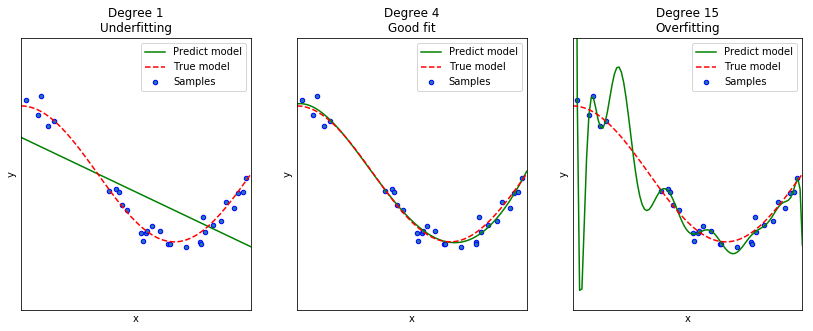
\includegraphics[scale=0.5]{chap3/image/overfitting.png}
    \end{center}
    \caption{overfitting và underfitting}
    \label{fig:overfitting}
    \end{figure}
\end{center}
Đường nét liền thể hiện \textit{mô hình dự đoán (predicted model)} , đường nét đứt thể hiện \textit{mô hình thực (true model)}, các chấm hình tròn là các điểm dữ liệu. Mô hình được xây dựng bằng hồi quy tuyến tính (\textit{linear regression}) với các feature là bậc mũ.\par
Ở hình thứ nhất chúng ta có thể thấy mô hình dự đoán là một hàm tuyến tính (bậc bằng 1) rất khác với mô hình thực, xa với các điểm dữ liệu. Hiện tượng này ta nói mô hình bị \textit{underfitting}.
Với mô hình dự đoán là đa thức bậc 4 chúng ta có thể thấy mô hình dự đoán xấp xỉ như mô hình thực (hình thứ 2). Trường hợp này ta nói mô hình phù hợp (\textit{good fit}). Ở hình thứ 3, khi ta tăng bậc đa thức lên thì mô hình dự đoán quá khớp với các điểm dữ liệu, gần như mọi điểm dữ liệu đều nằm trên mô hình. Tuy nhiên việc khớp hoàn toàn dữ liệu lại không hề tốt vì dữ liệu thường bị nhiễu và có thể khiến mô hình dự đoán bị nhiễu hơn. Trường hợp này ta nói mô hình bị\textit{ overfitting}. Để tránh vấn đề này xảy ra chúng ta có phương pháp khá là hữu dụng đó là \textit{regularization}.
%\subsubsection{Mối quan hệ giữa overfitting và hàm mát mát}
%  Như tôi đã trình bày phần trên, overfitting là hiện tượng mô hình quá khớp với tập dữ liệu huấn luyện có nghĩa là giá trị của hàm mất mát trên tập dữ liệu huấn luyện (\textit{$J_{train}$}) rất nhỏ. Nhưng khi đó giá trị của hàm mất trên tập dữ liệu test (\textit{$J_{test}$}) lại tăng lên gây ra mô hình mất đi sự tổng quát. 

\subsubsection{Một số phương pháp ngăn chặn overfitting}
Nhìn chung các phương pháp làm thay đổi nhỏ các tham số hay kiến trúc mô hình, chấp nhận hy sinh độ chính xác trong quá trình huấn luyện để giảm độ phức tạp của mô hình giúp tránh được hiện tượng overfitting mà vẫn giữ được tính tổng quát của mô hình.

\textbf{kỹ thuật regulazation}
\begin{enumerate}
\item Early stopping\\
  Khi ta dùng một phương pháp tối ưu hàm số để giảm thiểu giá trị mất mát thì \textit{$J_{train}, J_{test}$} sẽ cùng giảm theo thời gian nhưng nếu sau một thời gian \textit{$J_{test}$} tăng lên còn \textit{$J_{train}$} tiếp tục giảm thì đó là lúc bắt đầu dẫn đến overfitting. Cách đơn giản nhất để giảm thiểu overfitting đó là dừng huấn luyện tại ngay thời điểm bắt đầu overfitting và phương pháp này được gọi là \textit{early stopping}. Nếu ta có biểu đồ về sự thay đổi giá trị mất mát của trainning và testing như Hình \ref{fig:overfittingError} thì ta có thể thấy thời điểm sử dụng early stopping là vào khoảng epochs 50.

\begin{center}
 	\begin{figure}[H]
    \begin{center}
    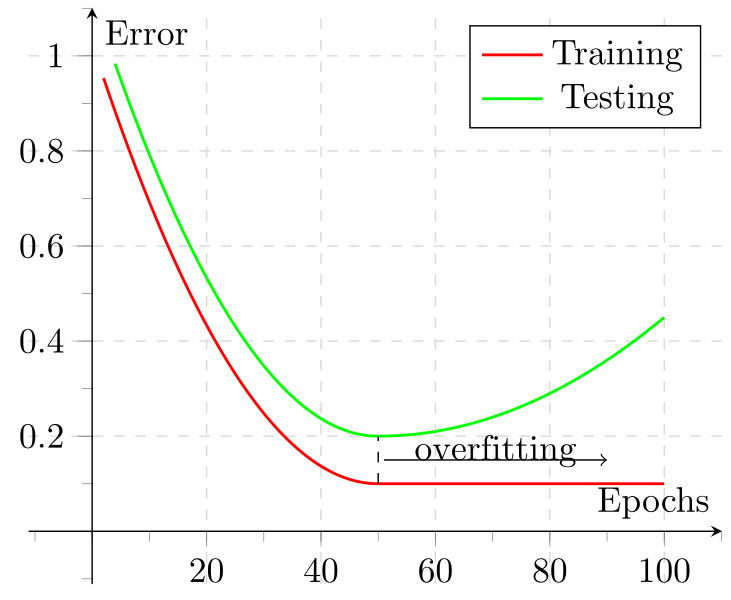
\includegraphics[scale=0.5]{chap3/image/overfittingError.png}
    \end{center}
    \caption{Early stopping}
    \label{fig:overfittingError}
    \end{figure}
\end{center}

\item Thêm số hạng vào hàm mất mát\\
  Một kỹ thuật regulazation phổ biến là thêm một số hạng vào hàm mất mát như sau:
\begin{equation}
	J_{reg}(\textbf{W}) = J(\textbf{W})+ \lambda R(\textbf{W})
\end{equation}
$J(\textbf{W})$ là hàm mất mát ban đầu và cụm $ \lambda R(\textbf{W})$  mới thêm vào là số hạng chính quy hoá (hay số hạng regularization) đóng vai trò như một biện pháp phạt lỗi (penalization).Trong đó, tham số chính quy hoá (\textit{regularizaton parameter}) $\lambda$ được chọn từ trước để cân bằng giữa $J(\textbf{W}) ~\text{và}~ R(\textbf{W})$. $\lambda$ càng lớn thì ta càng coi trọng $R(\textbf{W})$, ít coi trọng tham số cho hàm mất mát ban đầu hơn, dẫn tới việc các trọng số $\textbf{W}$ ít có ảnh hưởng tới mô hình hơn. Hay nói cách khác là mô hình bớt phức tạp đi giúp ta đỡ việc lỗi quá khớp.
$R(\textbf{W})$ thường có dạng như sau:
\begin{equation}
R(\textbf{W})= \frac{1}{p}\|\textbf{W}\|^p_p = \frac{1}{p}\sum^{n}_i |\textbf{W}|^p
\end{equation}
$p$ thường được chọn là 2 (\textit{$l_2 norm regularization$}) và 1 (\textit{$l_1 norm regularization$})\par
  Phương pháp chính quy hoá này còn có tên là phân rã trọng số (weight decay) vì nó khiến các hệ số trong $\textbf{W}$ không quá lớn, giúp tránh việc đầu ra phụ thuộc quá nhiều vào một đặc trưng nào đó.

\item Drop-out\\
Drop-out là một kĩ thuật Regularization để chống lại vấn đề overfitting. Cách dropout thực hiện là xoá bỏ một số unit trong các step training ứng với một giá trị xác suất $\textbf{p}$ cho trước. Các mạng mới sau khi áp dụng dropout được gọi là subsample. Thông thường xác suất ở layer input bằng 0.8 hay ta loại bỏ khoảng 20\% số unit, ở hidden layer thì xác suất là 0.5 có nghĩa là ta loại bỏ 50\% số unit ở layer sử dụng dropout.

\begin{center}
 	\begin{figure}[H]
    \begin{center}
    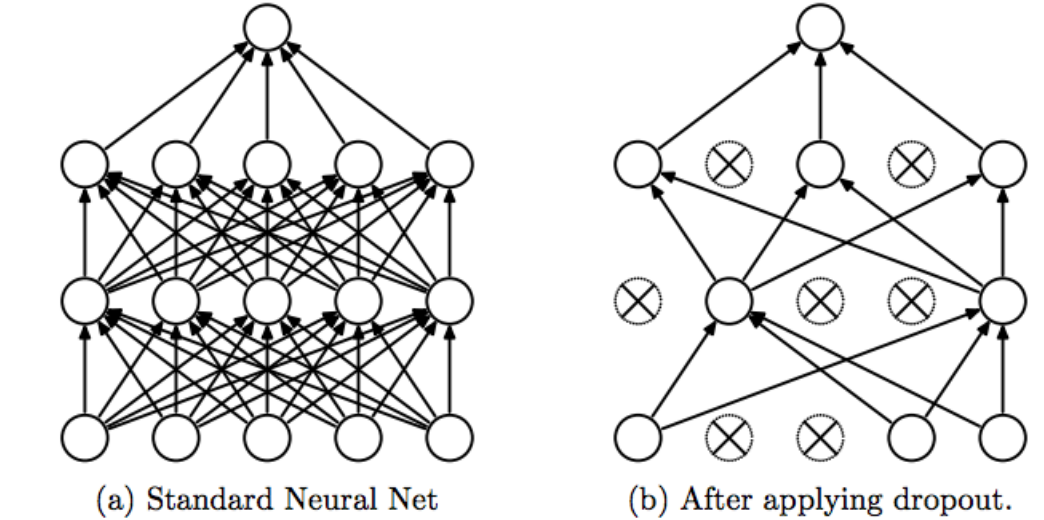
\includegraphics[scale=0.4]{chap3/image/dropout.png}
    \end{center}
    \caption{Dropout với p =0.5}
    \label{fig:dropout}
    \end{figure}
\end{center}

Cách hoạt động của dropout
\begin{itemize}
\item[•] Dropout được áp dụng trên một layer của mạng neural networks với một xác suất $\textbf{p}$ cho trước (có thể sử dụng nhiều Drop-Out khác nhau cho những layer khác nhau, nhưng trên 1 layer sẽ chỉ có 1 dropout)
\item[•] Tại mỗi step trong quá trình training, khi thực hiện feedforward đến layer sử dụng dropout, thay vì tính toán tất cả unit có trên layer, tại mỗi unit ta "gieo xúc xắc" với xác suất $p$ xem unit đó được tính (active) hay không được tính (deactive). Những unit active ta tính toán bình thường còn với những unit deactive thì ta set giá trị tại unit đó bằng 0
\item[•] Trong quá trình test thì tất cả các unit đều được active và chúng ta mong muốn đầu ra của các units giống với đầu ra mong đợi trong quá trình trainning. Ví dụ đầu ra của một unit (trước khi drôput) là $\textbf{a}$, khi áp dụng dropout thì đầu ra mong đợi của unit đó sẽ là $\textbf{p}\textbf{a} + (1-\textbf{p})0$, vì unit bị deactive thì giá trị của unit đó là 0. Do đó trong quá trình test chúng ta điều chỉnh đầu ra $\textbf{a} \to \textbf{p}\textbf{a}$ để  giống với đầu ra mong đợi.
\end{itemize} 
Thời gian test khá là quan trọng nên nếu chúng ta điều chỉnh đầu ra ở các layer áp dụng dropout thì hiệu suất test sẽ bị giảm đi. Vì thế thay vì chỉnh trong quá trình test thì chúng ta sẽ thực hiện việc này trong quá trình trainning. Ta sẽ lấy \textit{dropout mask} (vector xác suất được khởi tạo ngẫu nhiên, tại vị trí có giá trị nhỏ hơn $p$ sẽ được giữ nguyên còn lớn hơn $p$ sẽ set lại giá trị vị trí đó là 0) chia cho $p$ trong quá trình trainning. Trường hợp này được gọi là \textit{inverted dropout}.
\end{enumerate}

\subsection{Dữ liệu}
Dữ liệu thường được chia làm ba phần: tập huấn luyện, tập đánh giá, tập kiểm tra. Tỉ lệ thường được lấy của các tập dữ liệu: tập kiểm tra bằng 20\% tổng dữ liệu, tập huấn luyện bằng 80\% tổng dữ liệu, tập đánh giá bằng 20\% tập huấn luyện. Tuy nhiên vì tỉ lệ được so với số lượng dữ liệu ta thu thập được nên không phải lúc nào cũng giống nhau. Nếu thu thập được nhiều dữ liệu thì ta có thể tăng tỉ lệ tập huấn luyện và giảm với tập kiểm tra, đánh giá. Một số vai trò chính của các tập:
\begin{itemize}
\item[•]Tập huấn luyện đóng vai trò làm đầu vào cho mạng nơ-ron giúp tìm ra được các trọng số phù hợp với dữ liệu cần đánh giá.
\item[•]Tập đánh giá sẽ được chạy trong quá trình huấn luyện, sau mỗi epoch và giúp đánh giá mô hình đã tốt chưa, liệu có cần thay đổi giá trị của các tham số.
\item[•]Tập kiểm tra cũng giống như tập đánh giá, cho ta biết độ chính xác của mô hình đối với các dữ liệu không có trong tập huấn luyện nhưng được chạy khi mô hình đã được huấn luyện.
\end{itemize}
Dữ liệu cần được chuẩn hóa trước khi đưa vào mạng huấn luyện, ví dụ như nên đưa dữ liệu về khoảng [0,1] để tiện cho việc tính toán và các feature không bị chênh lệch nhau hay nếu dữ liệu là ảnh thì cần đưa về cùng kích thước.
\section{Mạng nơ-ron tích chập}

\subsection{Tổng quan}
  \textit{Mạng nơ-ron tích chập}, có tên tiếng anh  Convolutional Neural Network và được viết tắt là CNN, là một trong những mô hình học sâu tiên tiến giúp xây dựng được những hệ thống thông minh với độ chính xác cao. Trong khóa luận này, tôi sẽ trình bày về tổng quan về mạng nơ-ron tích chập và ứng dụng CNN cho bài toán phân loại biển báo giao thông.\par
Mạng nơ-ron tích chập lấy cảm hứng từ xử lý ảnh nên đầu vào và các lớp của CNNs có dạng như một bức ảnh, là các ma trận chứ không có dạng vector như mạng nơ-ron thông thường. Cụ thể, một bức ảnh sau khi số hoá có dạng \textit{dài $\times$ rộng $\times$ sâu} (dài: số lượng điểm ảnh trên chiều rộng, rộng : số lượng điểm ảnh trên chiều cao, depth: số lượng kênh chẳng hạn như RGB có 3 kênh đại diện cho mức độ của 3 màu Đỏ, Lục, Lam). Mô hình được mô tả ở Hình \ref{fig:conv}.

\begin{center}
\begin{figure}[H]

\begin{center}
\subfloat[mạng nơron thông thường]
  {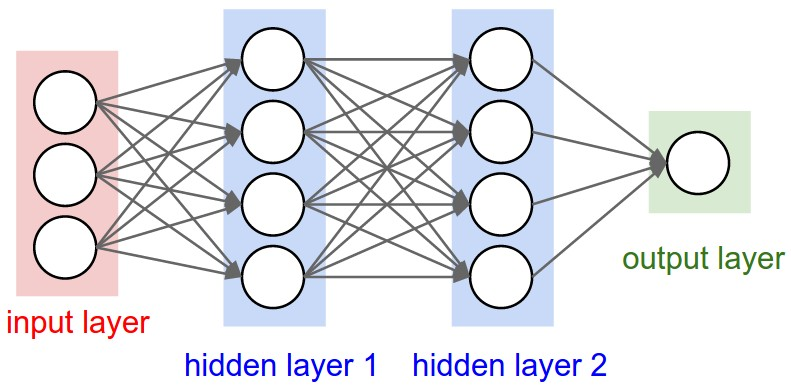
\includegraphics[width=.3\linewidth]{chap3/image/cnn/architectureNNs}}
\subfloat[mạng nơron tích chập]
  {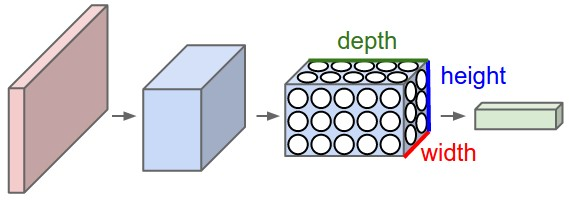
\includegraphics[width=.3\linewidth]{chap3/image/cnn/architectureCNN}}
  \label{fig:conv}
\caption{Kiến trúc hai mạng}
\end{center}

\end{figure}
\end{center}

Một mạng CNNs đơn giản có ba lớp chính: lớp tích chập (\textit{convolutional layer}), lớp giảm số chiều (\textit{pooling layer}), lớp fully-connected. Các lớp convolutional và lớp pooling được xếp xen kẽ nhau Hình \ref{fig:convNetArch}.
\begin{center}
\begin{figure}[H]
	\begin{center}
		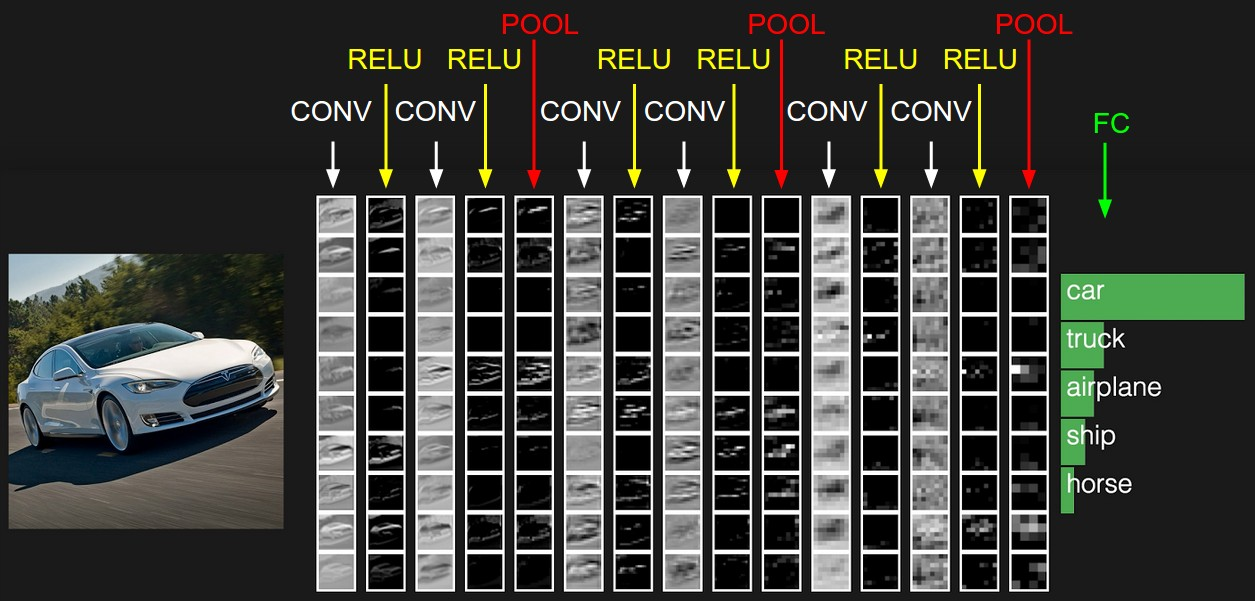
\includegraphics[scale=0.2]{chap3/image/cnn/convnet.jpeg}
	\end{center}
	\caption{ví dụ về kiến trúc của ConvNets}
	
\label{fig:convNetArch}
\end{figure}
\end{center}
\subsection{Lớp tích chập - Convolutional layer}
  \textit{Convolution layer} là khối cốt lõi, cơ bản của ConvNets, lớp này chủ yếu nặng về việc tính toán. Lớp này chính là nơi thể hiện tư tưởng ban đầu của mạng nơron tích chập. Thay vì kết nối toàn bộ điểm ảnh, lớp này sẽ sử dụng \textit{bộ lọc (filter)} áp vào một vùng trong ảnh và tiến hành tính element-wise giữa bộ lọc và \textit{vùng tiếp nhận cục bộ (local receptive filter)}. Sau đó ta dùng phương pháp \textit{cửa sổ trượt (sliding window)} để bộ lọc quét hết các vùng trong ảnh. 
\begin{figure}[H]

\subfloat[\label{fig:slide1_1}]
  {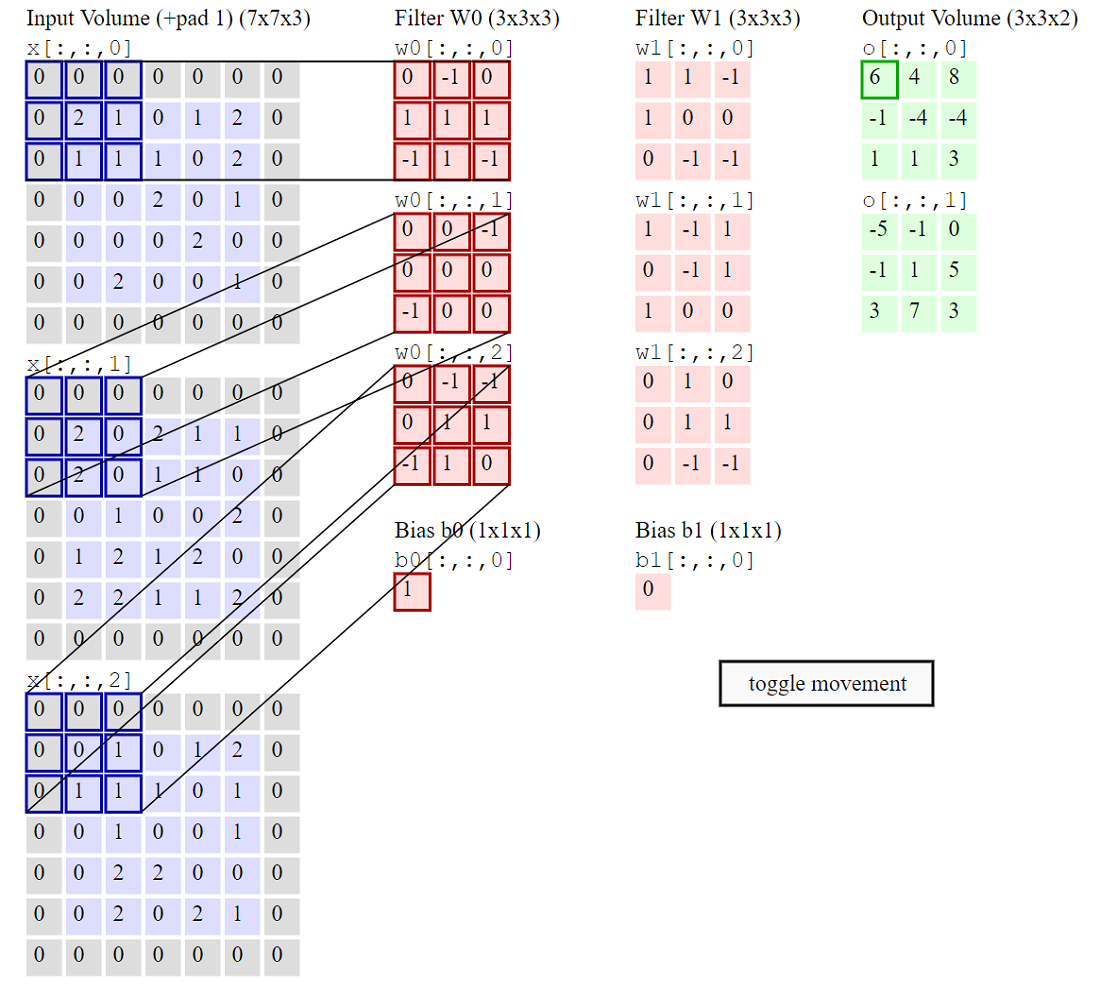
\includegraphics[width=.3\linewidth]{chap3/image/cnn/slide1_1.png}}\hfill
\subfloat[\label{fig:slide1_2}]
  {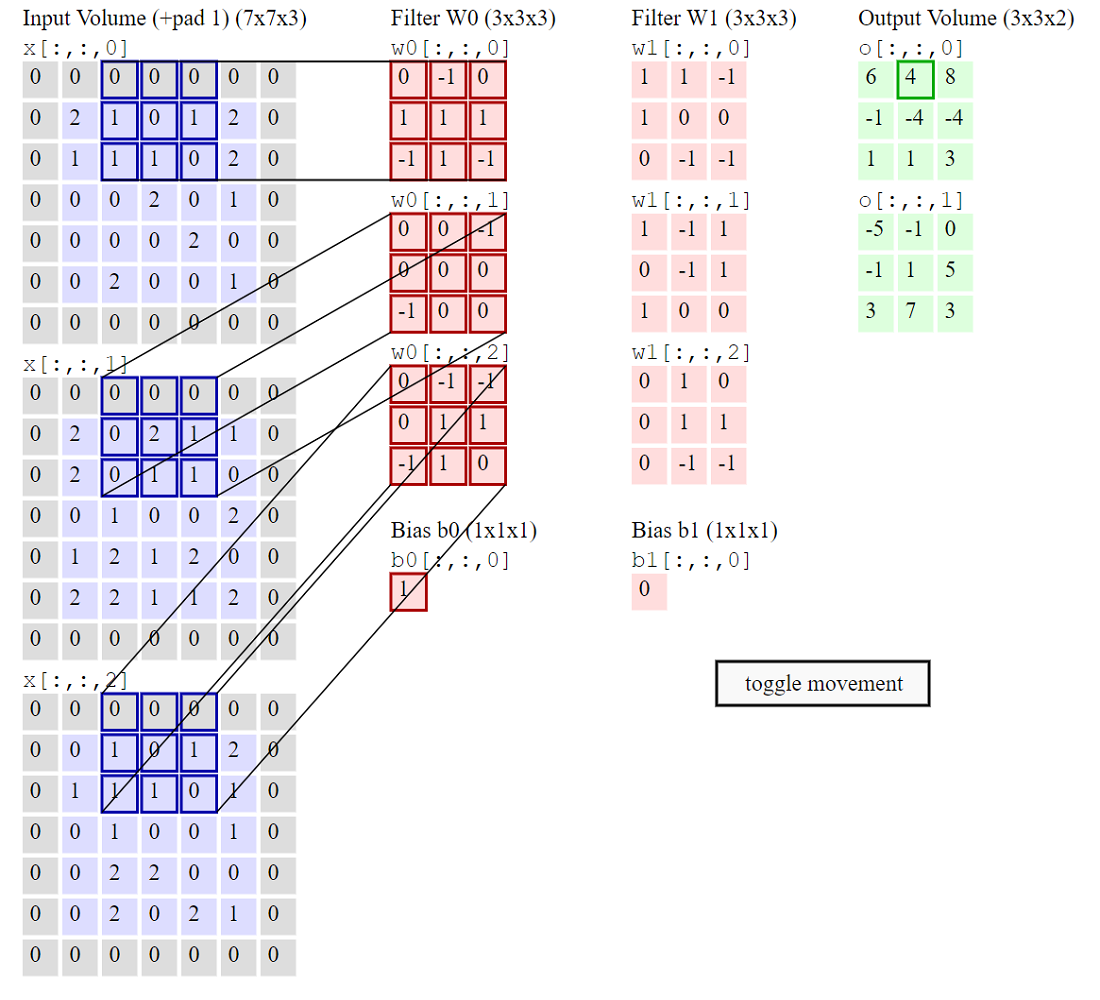
\includegraphics[width=.3\linewidth]{chap3/image/cnn/slide1_2.png}}\hfill
\subfloat[\label{fig:slide1_3}]
  {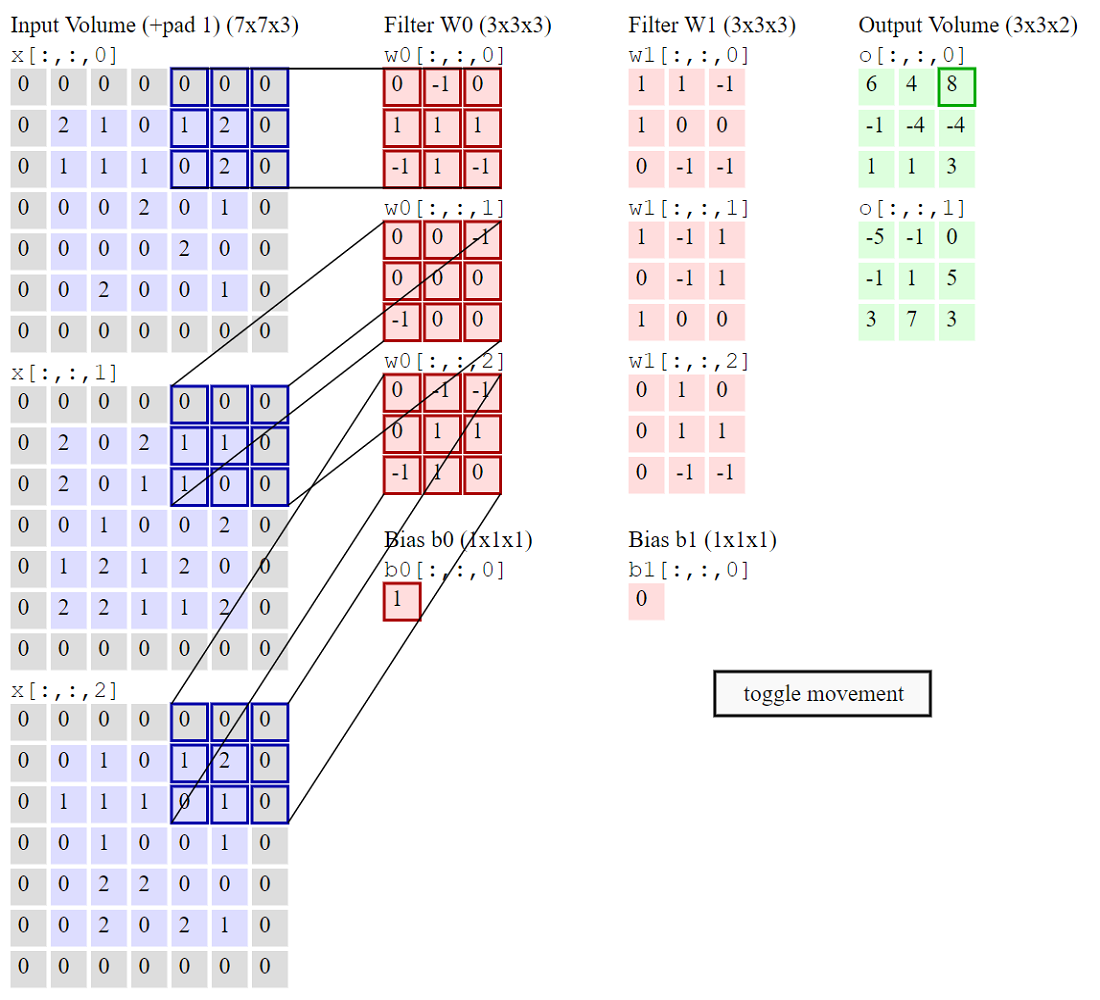
\includegraphics[width=.3\linewidth]{chap3/image/cnn/slide1_3.png}}\\
\subfloat[\label{fig:slide2_1}]
  {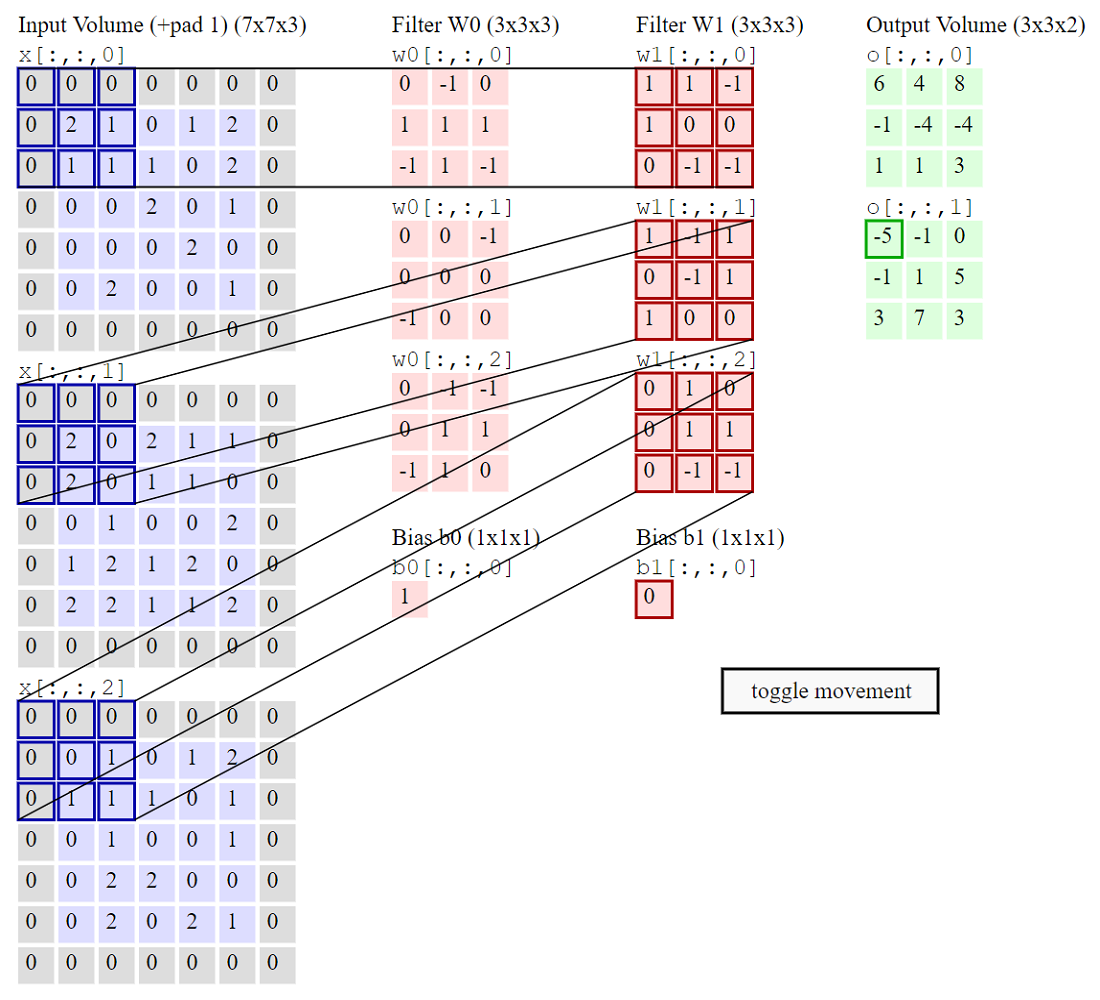
\includegraphics[width=.3\linewidth]{chap3/image/cnn/slide2_1.png}}\hfill
\subfloat[\label{fig:slide2_2}]
  {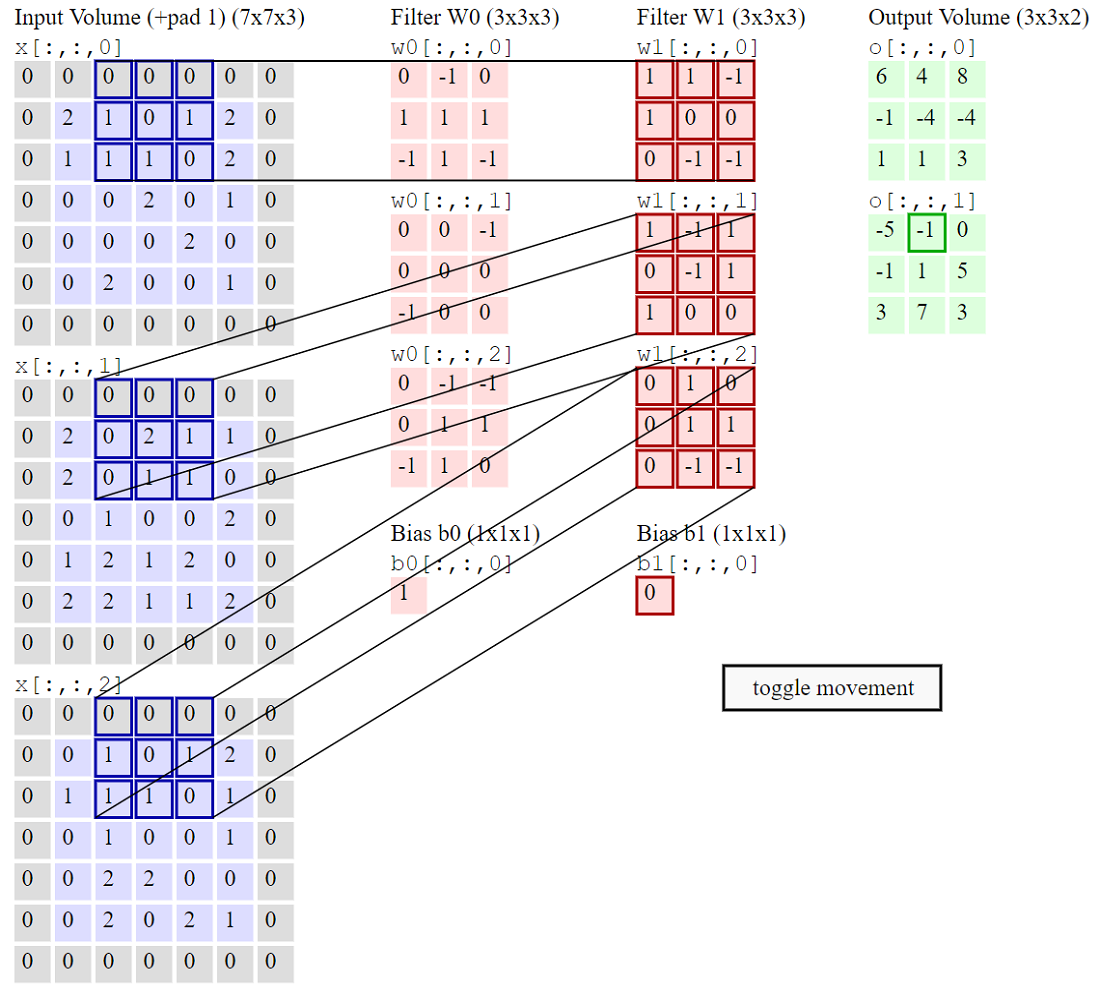
\includegraphics[width=.3\linewidth]{chap3/image/cnn/slide2_2.png}}\hfill
\subfloat[\label{fig:slide2_3}]
  {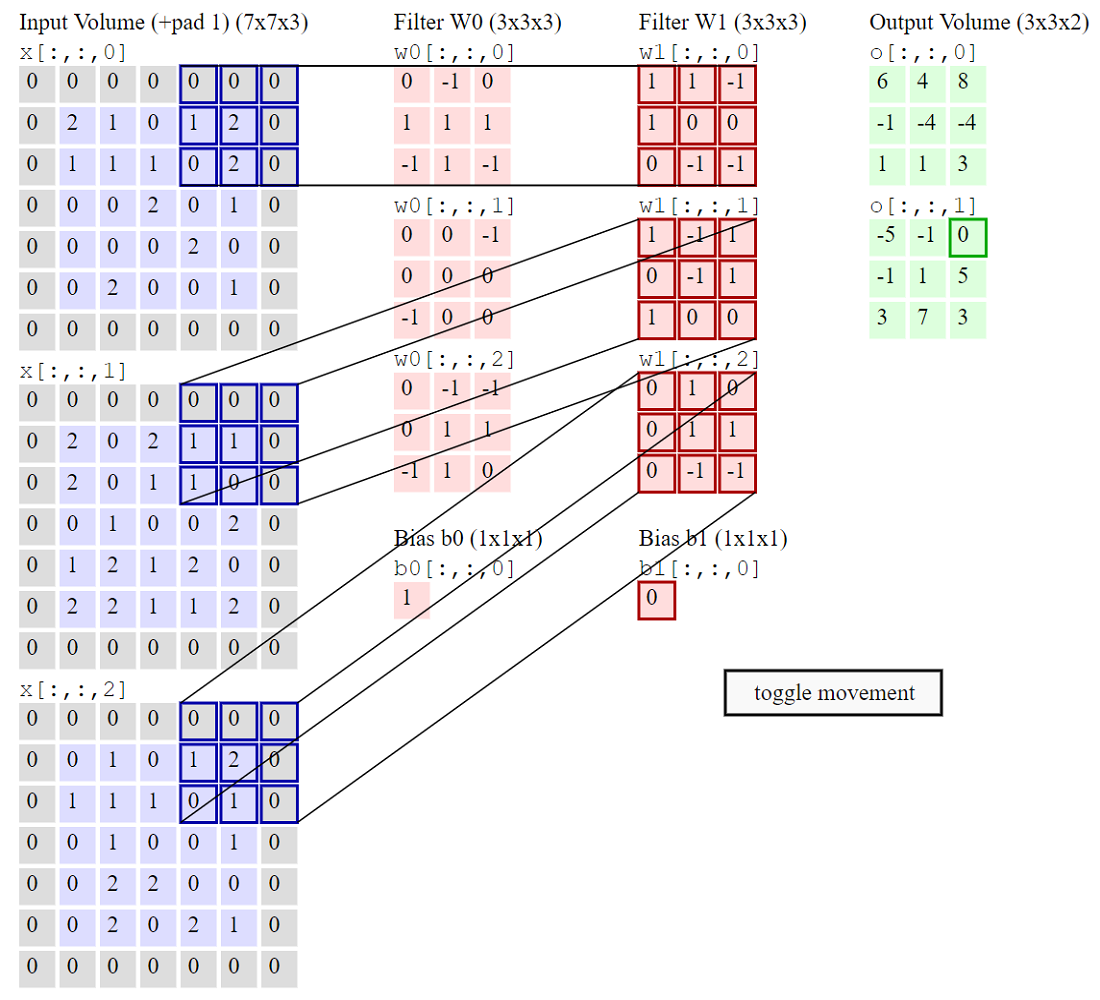
\includegraphics[width=.3\linewidth]{chap3/image/cnn/slide2_3.png}}
\caption{Tính toán trong lớp tích chập}
\label{fig:tinhtoanConv}
\end{figure}
\subsubsection{Bộ lọc}
  Bộ lọc hay còn gọi là filter hoặc kennel, là các ma trận có kích thước nhỏ ($3\times 3, 5\times 5, 7\time7, \ldots$) giúp ta thay đổi các giá trị đầu vào dựa vào các giá trị lân cận theo một nguyên tắc, công thức nào đó. Tùy theo đầu vào của bài toán thì kích thước của bộ lọc được thay đổi để phù hợp với hình dạng của đầu vào. Chúng ta sẽ rõ hơn khi xem hình \ref{fig:filter}, ta có ma trận $I$ là ma trận đầu vào, ma trận K là bộ lọc, ma trận I*K là ma trận kết quả với mỗi phần tử là kết quả của phép tính element-wise giữa bộ lọc và vùng re
\begin{center}
\begin{figure}[htp]
	\begin{center}
		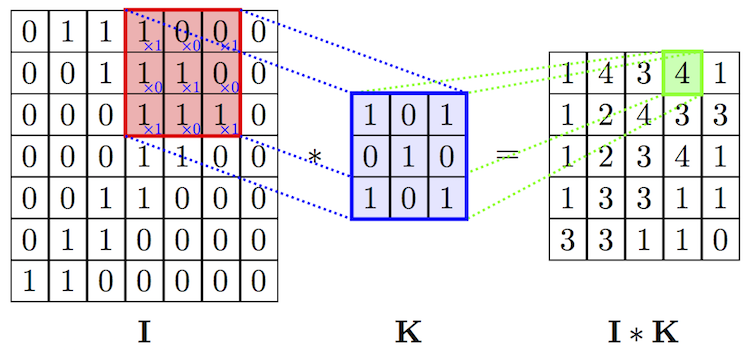
\includegraphics[scale=1.2]{chap3/image/cnn/minhHoaTichChap.png}
	\end{center}
	\caption{Bộ lọc - filter}
	\label{fig:filter}
\end{figure}
\end{center}
Nhưng khi với đầu vào giống như Hình \ref{fig:tinhtoanConv} thì kích thước bộ lọc là ma trận 3 chiều.
  Kích thước của các filter thường là $d\times3\times3$, $d\times5\times5$, $d\times7\times7$  hoặc $d\times11\times11$, trong đó $d$ là chiều sâu của filter, hai tham số tiếp theo thể hiện chiều rộng và chiều cao của filter. Chú ý rằng chiều sâu của filter luôn luôn bằng chiều sâu của đầu vào.
\subsubsection{Cửa sổ trượt}
  Cửa sổ trượt hay còn có tên tiếng anh là sliding window là ta chọn một "cửa sổ" có kích thước nhỏ hơn kích thước đầu vào và trượt cửa sổ đó trên đầu vào theo chiều ngang và chiều dọc. Các bước trượt là khoảng cách mà ta dịch chuyển filter trên đầu vào và đó gọi là \textit{stride}, ký hiệu là $s$. Ví dụ như Hình \ref{fig:slidingwindow}, ta có đầu vào kích thước là $5\times5$, cửa sổ có kích thước là $3\times3$ và tại mỗi bước trượt cửa sổ dịch chuyển đi một đơn vị, do đó stride bằng 1.
\begin{center}
\begin{figure}[htp]
	\begin{center}
		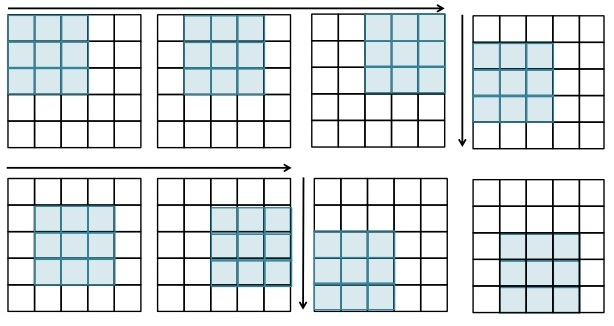
\includegraphics[scale=1]{chap3/image/cnn/slidingwindow.jpg}
	\end{center}
	\caption{Sliding window}
	\label{fig:slidingwindow}
\end{figure}
\end{center}
\subsubsection{Cách thức hoạt động}
Theo Hình \ref{fig:tinhtoanConv} ta có kích thước đầu vào là $7 \times 7\times 3$, stride bằng 2, kích thước filter là  $2\times 3\times 3 \times 3$ với 2 là số \textit{channel} (số chanel sẽ là chiều sâu output chúng ta mong muốn). Tại Hình \ref{fig:slide1_1} ta  thực hiện phép tính... tương ứng giữa receptive filter, $filter ~W0$ tại tất cả các độ sâu, kết quả được cộng thêm $bias$ rồi lưu vào ma trận output vị trí đầu tiên của đầu ra. Sau đó ta thực hiện cách tính toán trên kết hợp sliding window với stride bằng 2 và filter là $filter W0$, kết quả ta thu được là ma trận output thứ nhất, các Hình \ref{fig:slide1_1}, \ref{fig:slide1_2}, \ref{fig:slide1_3} mô tả giai đoạn này. Và tương tự như trên ta thực hiện với $filter ~W1$ theo Hình \ref{fig:slide2_1}, \ref{fig:slide2_2}, \ref{fig:slide2_3} ta thu được kết quả là ma trận thứ hai tại output. Như vậy nếu ta có càng nhiều channel thì chiều sâu output của chúng ta càng lớn. \par

Nếu như đầu ta chỉ tính trên kích thước đầu vào thì với filter $3\times 3$ và stride bằng 2 thì ta chỉ trượt được hai lần và đến hàng, cột thứ 5 của đầu vào còn giá trị tại hàng, cột thứ 6, 7 sẽ không được tính. Vì thế chúng ta thêm vào ma trận đầu vào các hàng và cột đối xứng với giá trị bằng 0 để không ảnh hưởng đến đầu vào mà khi đó ta sẽ quét được hết các giá trị của đầu vào. Cách này được gọi là \textit{zero padding}. Như ở ví dụ trên ta thấy đầu vào được bao quanh bởi các số 0 và kích thước tăng thành $8 \times 8$, đó là ta áp dụng zero padding với p=1.\\
Ta có công thức để tính toán kích thước đầu ra như sau:
\begin{itemize}
	\item Kích thước đầu vào \textbf{$W_1$} x \textbf{$H_1$} x \textbf{$D_1$} (rộng x cao x sâu)
	\item Kích thước của filter \textbf{$F$}
	\item Số channel \textbf{$K$}
	\item Tốc độ trượt \textbf{$S$}
	\item Giá trị của zero-padding \textbf{$P$}
	\item Kích thước đầu ra \textbf{$W_2$} x \textbf{$H_2$} x \textbf{$D_2$}:
	\begin{itemize}
		\item[+]  \textbf{$W_2 = (W_1 - F+ 2P)/S +1$}
		\item[+] \textbf{$H_2 = (H_1 - F+ 2P)/S +1$}
		\item[+] \textbf{$D_2 = K$}
	\end{itemize}	 
\end{itemize}	

\begin{center}
\begin{figure}[htp]
	\begin{center}
		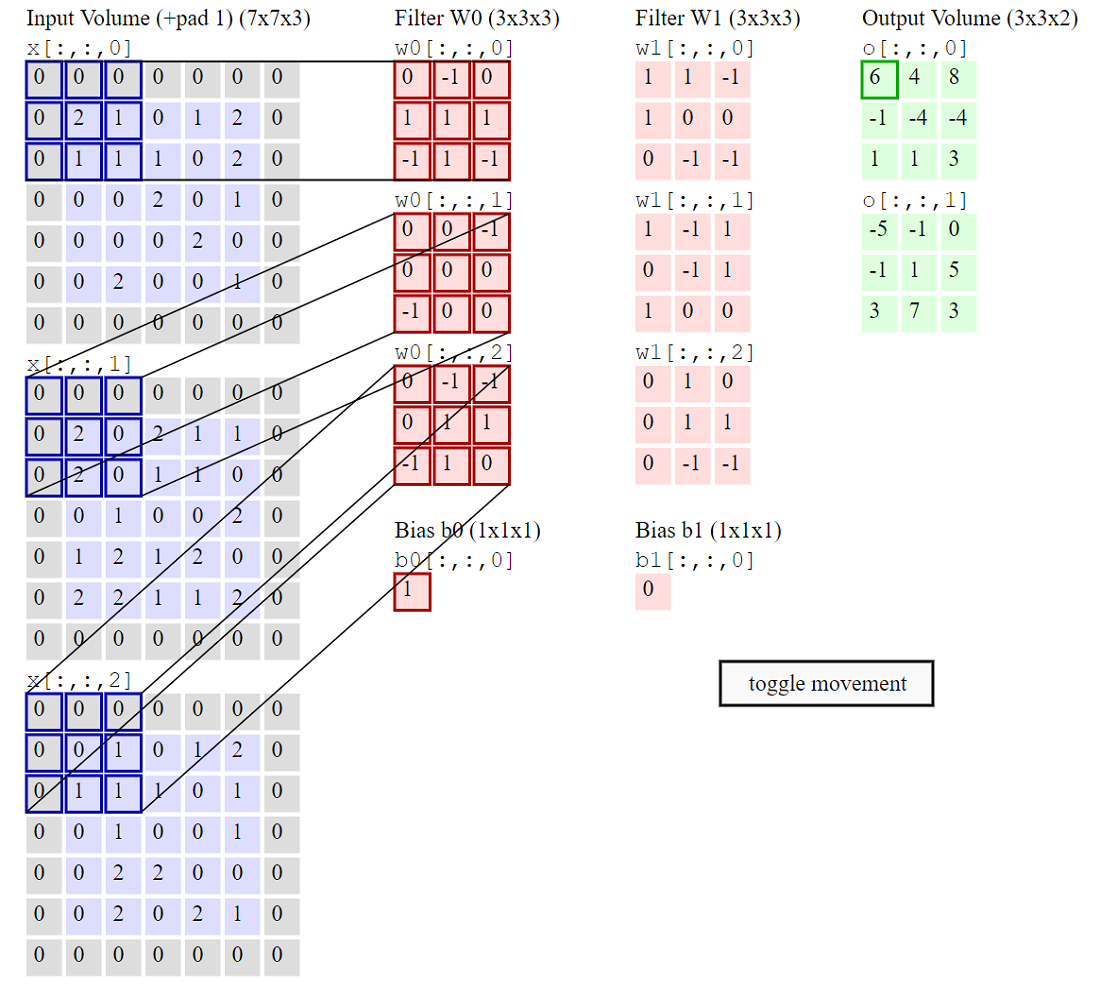
\includegraphics[scale=0.4]{chap3/image/cnn/slide1_1.png}
	\end{center}
	\caption{Ví dụ về tính toán kích thước đầu ra}
	\label{fig:minhhoatichchap2}
\end{figure}
\end{center}
  Giả sử ta có thông số như hình \ref{fig:minhhoatichchap2} với kích thước đầo vào là $7\times7\times3$ tương đương $W=H=7,~ D_1=3$;stride $S=3$; kích thước filter là $2\times 3\times 3 \times 3$ hay $F=3$ và số channel $K=2$. Theo công thức ta tính được $(W_1 - F+ 2P)/S$ không phải là số nguyên do đó ta cần thêm padding để giá trị này là số nguyên. Ta chọn $P=1$ vì $(7-3+2\times 1)/3 +1$ là số nguyên. Như vậy ta tính được kích thước đầu ra sẽ là $3\times3\times2$. \par
Một phần quan trọng của layer này đó là hàm activation, hàm này được tính với đầu vào là kết quả sau khi thực hiện tích chập. Và ReLU thường được chọn là hàm activation do tính đơn giản của nó. Nhiệm vụ của nó là chuyển toàn bộ giá trị âm trong kết quả sau khi tích chập thành 0. Ý nghĩa của cách cài đặt này chính là tạo nên tính phi tuyến cho mô hình. 
\subsection{Lớp giảm số chiều -  pooling layer}
  \textit{Lớp giảm số chiều (pooling layer)} trong mạng CNNs thực hiện công việc loại bỏ bớt những thông tin không cần thiết sau khi thực hiện tích chập và được chèn giữa các lớp convolutional với nhau hoặc sau một tập lớp convolutional. Nó có vai trò giảm kích thước dữ liệu. Với một bức ảnh kích thước lớn qua nhiều lớp pooling sẽ được thu nhỏ lại tuy nhiên vẫn giữ được những đặc trưng cần cho việc nhận dạng (thông qua cách lấy mẫu). Việc giảm kích thước dữ liệu sẽ làm giảm lượng tham số, tăng hiệu quả tính toán và góp phần kiểm soát hiện tượng quá khớp (overfitting). Tuy nhiên nếu lạm dụng loại layer này cũng có thể khiến data đi qua bị mất dữ liệu.\par
\textbf{Cách thức hoạt động}: Pooling layer sử dụng sliding window và tại mỗi cửa sổ trượt trên đầu vào chỉ có một giá trị được xem là giá trị đại diện cho thông tin ảnh tại vùng đó (giá trị mẫu) được giữ lại và đó gọi là tiến hành lấy mẫu (\textit{subsampling}). Các phương thức lấy phổ biến trong pooling layer là \textit{Max pooling} (lấy giá trị lớn nhất), \textit{Min pooling} (lấy giá trị nhỏ nhất) và \textit{Average Pooling} (lấy giá trị trung bình). Hình \ref{fig:pool} mô tả tiến hành lấy mẫu bằng max pooling.

\begin{center}
\begin{figure}[H]
	\begin{center}
		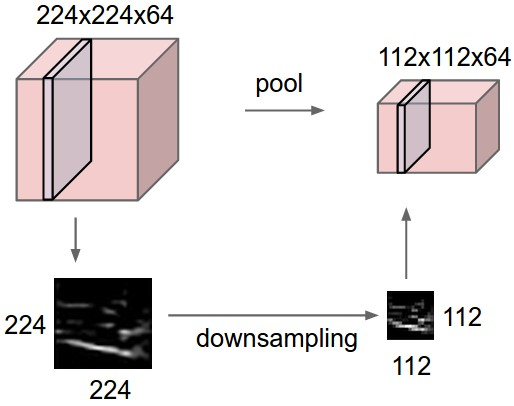
\includegraphics[scale=0.5]{chap3/image/cnn/poolEx.jpeg}
	\end{center}
	\caption{Minh họa giảm số chiều}
	\label{fig:pool}
\end{figure}
\end{center}
Ví dụ ta có ma trận đầu vào $4\times 4$  như hình \ref{fig:poolExample}, với kích thước cửa sổ áp dụng cho slidiing window là $2\times 2$ và stride = 2, điều này tương đương với việc ta chia ma trận đầu vào thành 4 ma trận con với kích thước là $2\times2$.  Phương thức ta áp dụng tại đây là max pooling, do đó tại mỗi cửa sổ khi ta áp vào đầu vào thì ta sẽ chọn giá trị lớn nhất làm đại diện cho cửa sổ đó và ta thu được kết quả là ma trận $2\times2$ bên tay phải.
\begin{center}
\begin{figure}[htp]
	\begin{center}
		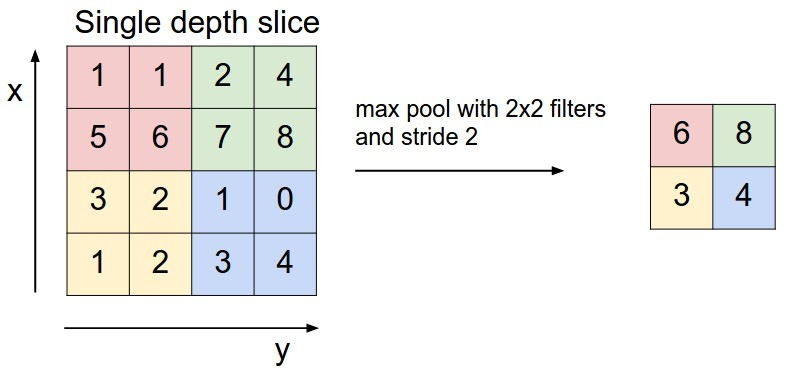
\includegraphics[scale=0.5]{chap3/image/cnn/maxpoolEx.jpeg}
	\end{center}
	\caption{Max pooling}
	\label{fig:poolExample}
\end{figure}
\end{center}
  Ta rút ra được công thức tính kích thước đầu ra cho lớp này như sau:
\begin{itemize}
	\item Kích thước đầu vào \textbf{$W_1$} x \textbf{$H_1$} x \textbf{$D_1$} (rộng x cao x sâu),
	\item Kích thước cửa sổ \textbf{$F$},	
	\item Tốc độ trượt \textbf{$S$}
	\item Kích thước đầu ra \textbf{$W_2$} x \textbf{$H_2$} x \textbf{$D_2$}:
	\begin{itemize}
		\item  \textbf{$W_2 = (W_1 - F)/S +1$}
		\item  \textbf{$H_2 = (H_1 - F)/S +1$}
		\item \textbf{$D_2 = D_1$}
	\end{itemize}	 
\end{itemize}
Chú ý rằng chúng ta không thường xuyên sử dụng $zero~padding$ cho lớp này.
\subsection{Lớp Fully-Connected (Fully-Connected layer)}
  Sau khi ảnh được xử lý và trích xuất đặc trưng bằng các lớp convolutional, pooling thì ta sẽ làm phẳng (flatten) output cuối cùng của giai đoạn trước đó và áp dụng mạng nơron truyền thẳng với input là dữ liệu ta vừa làm phẳng. Hay nói cách khác Fully-Connected chính là một mạng nơron được gắn vào phần cuối của CNNs với input là đầu ra của các lớp trước đó. Nó đóng vai trò như một mô hình phân lớp và tiến hành dựa trên dữ liệu đã được xử lý ở các lớp trước đó.
\section{Tổng kết}
  Dưới đây là một mô hình mạng CNNs kết hợp giữa các layer với nhau với cấu trúc như sau: Conv $\to$ Max-pool $\to$ Conv (giữ nguyên kích thước) $\to$ Max-pool $\to$ Conv (giữ nguyên kích thước) $\to$ Conv (giữ nguyên kích thước) $\to$ Conv (giữ nguyên kích thước) $\to$ Max-pool $\to$ Flatten $\to$ FC . Kích thước các lớp được thể hiện tại Hình \ref{fig:CNN}.
\begin{center}
\begin{figure}[H]
	\begin{center}
		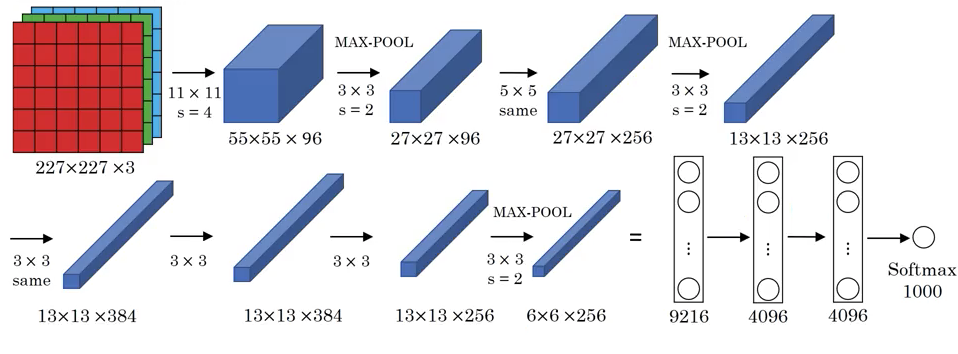
\includegraphics[scale=0.5]{chap3/image/cnn/CNN.png}
	\end{center}
	\caption{Ví dụ cấu trúc mạng CNNs}
	\label{fig:CNN}
\end{figure}
\end{center}
